\documentclass{AISB2008}
\usepackage{times}
\usepackage{graphicx}
\usepackage{latexsym}
\usepackage{graphicx}
\usepackage[space]{grffile}
\usepackage{latexsym}
\usepackage{textcomp}
\usepackage{longtable}
\usepackage{tabulary}
\usepackage{booktabs,array,multirow}
\usepackage{amsfonts,amsmath,amssymb}
\providecommand\citet{\cite}
\providecommand\citep{\cite}
\providecommand\citealt{\cite}
\usepackage{url}
\usepackage{hyperref}
\hypersetup{colorlinks=false,pdfborder={0 0 0}}
\usepackage{etoolbox}
\makeatletter
\patchcmd\@combinedblfloats{\box\@outputbox}{\unvbox\@outputbox}{}{%
  \errmessage{\noexpand\@combinedblfloats could not be patched}%
}
\makeatother
% You can conditionalize code for latexml or normal latex using this.
\newif\iflatexml\latexmlfalse
\AtBeginDocument{\DeclareGraphicsExtensions{.pdf,.PDF,.eps,.EPS,.png,.PNG,.tif,.TIF,.jpg,.JPG,.jpeg,.JPEG}}

\usepackage[utf8]{inputenc}
\usepackage[ngerman,english]{babel}


\usepackage{siunitx}
\usepackage{natbib}
\usepackage{booktabs}
\begin{document}

\title{A Data-Driven Evaluation of Delays in Criminal Prosecution}


\author{Hrafnkell Hjörleifsson \institute{New York University Center for Urban Science \& Progress}\\
  \and Michelle Ho\institute{New York University Center for Urban Science \& Progress}\\
  \and Christopher Prince\institute{New York University Center for Urban Science \& Progress}\\
  \and Achilles Edwin Alfred Saxby\institute{New York University Center for Urban Science \& Progress}\\
  \and BetaGov \institute{New York University}\\
   \and Gregory G. Dobler\institute{New York University  Center for Urban Science \& Progress}\\
   \and Federica B Bianco\institute{New York University  Center for Urban Science \& Progress}\\
   \and Santa Clara District Attorney's office}


\maketitle




\textbf{Abstract}

The District Attorney's office of Santa Clara County, California has
observed long durations for their prosecution processes. It is
interested in assessing the drivers of prosecutorial delays and
determining whether there is evidence of disparate treatment of accused
individuals in pre-trial detention and criminal charging practices. A
recent report from the county's civil grand jury found that only 47\% of
cases from 2013 were resolved in less than year, far less than the
statwide average of 88\%. We describe a visualization tool and
analytical models to identify factors affecting delays in the
prosecutorial process and any characteristics that are associated with
disparate treatment of defendants. Using prosecutorial data from January
through June of 2014, we find that the time to close the initial phase
of prosecution (the entering of a plea), the initial plea entered, the
type of court in which a defendant is tried and the main charged offense
are important predictors of whether a case will extend beyond one year.
Durations for prosecution are found not significantly different for
different racial and ethnic population, and do not appear as important
features in our modeling to predict case durations longer than one year.
Further, we find that, in this data, 81\% of felony cases were resolved
in less than one year, far greater than the value reported by the civil
grand jury.p

\large{Authors}


{\it NYU Center for Urban Science and Progress} \\

Mentors: Federica B. Bianco {\it NYU Center for Urban Science and Progress} \\Sponsors:  NYU BetaGov/Litmus and the Santa Clara District Attorney's Office.}  

\section{Prior Work on Evaluating Prosecutorial Efficiency }

 \subsection{Existing measurements of prosecution performance} 

Previous studies have examined case-processing time as a standardized
measurement allowing comparison across jurisdictions
\hyperref[csl:6]{(Klemm 1986)}. In order to use case-processing time,
researchers first must subdivide case timelines into appropriate time
frames and reduce the scope to time under the control of the court
system \hyperref[csl:7]{(Neubauer 1983)}. Early studies have also
shown that case complexities such as prior convictions, mandatory
minimums, and the number of defendants in specific jurisdictions may
contribute to the length of a case \hyperref[csl:8]{(Luskin and Luskin
  1986}; \hyperref[csl:9]{Walsh et al. 2015)}. These findings align
with the expectations of prosecutors at the SCC District Attorney's
office and form the basis for our capstone project.

In recent years, there have been other data-driven efforts to evaluate
and compare court system performance. One such effort is
\hyperref[csl:5]{({Measures for Justice} 2017)}, an initiative to
aggregate and compare the performance of criminal justice systems from
arrest to post-conviction for the entire country via an interactive
public dashboard. One of the largest challenges is that criminal
justice data are neither recorded uniformly across local jurisdictions
nor are publicly available. The solution from Measures for Justice is
to reach out individually to jurisdictions to obtain data and then
create standardized core measurements for evaluating performance.

In addition to parsing and understanding case timelines, another
motivation of this capstone is to determine whether the addition of
defendant characteristics can explain delays in resolution, which
would indicate the presence of disparities. It is widely perceived
that race/ethnic disparities pervade the criminal justice system, and
much research has been conducted on biases at the point of arrest and
police interaction \hyperref[csl:10]{(Ross 2015)}. However, no
previous work has found the presence of racial disparities in
criminal-case processing times.

\subsection{Previous analytical techniques}

Machine learning models can be helpful in decision making in the presence of a large amount of data. To be adopted by policy makers, though, they must be easily interpretable and cost-effective. Previous studies on the topic of time to disposition is dominated by linear regression and basic exploratory analysis. The use of machine learning techniques in the field of criminology is just beginning to emerge. Use of tree-based classifiers to model the outcomes of cases \hyperref[csl:1]{(Katz, Ii, and Blackman 2017)} and advanced techniques in modeling cost-effective treatment regimes to optimize bail decisions \hyperref[csl:2]{(Lakkaraju and Rudin 2016)} focus on accuracy of prediction and optimization. The employment of advanced models on case processing time could help inform prosecutors in making decisions that both minimize case length and prioritize fair outcomes.


\section{Data}\label{data}

\subsection{Data sources}\label{data-sources}

The data used in this project were obtained from the DA's office of SCC,
which stores its case information in a case management database called
CIBERlaw. We received data for all felony cases charged by the SCC DA's
office between January 1st and June 30th 2014 for adult defendants. The
reason for this specific timeframe is twofold. Firstly, on the 5th of
November 2014, Proposition 47 was passed in a referendum in California.
With Proposition 47 certain non-violent drug and property crimes in the
state were reclassified as misdemeanors instead of felonies. It was at
the request of SCC DA's office that the time period selected would be
one prior to these changes. Secondly, to maximise the proportion of
cases concluded at the time of research it is preferrable to examine a
not too recent time period. The data arrived as four separate datasets:

\begin{itemize}
\tightlist
\item
  \textbf{Case Information}: Case Information has the base information
  of each case: case ID numbers, defendant ID numbers, the time a case
  is logged, and other basic information for each case. It also has
  demographic information for each defendant: race/ethnicity, gender,
  age and zipcode of residence. The dataset contains 4,794 observations,
  with the same number of unique defendant ID's and 4,405 unique case
  ID's.
\item
  \textbf{Defendant Charges}: Defendant charges has information on the
  charges facing defendants relayed in penal codes. It contains 34,421
  observations with 15,668 unique case IDs.
\item
  \textbf{Charge Enhancements}: Charge enhancements has limited
  information on prior convictions of defendants as well as enhancements
  on current charges. When a charge (from Defendant Charges dataset) is
  enhanced it mandates harsher sentancing. An examle of this is if a
  driver is charged for driving under the influence of alcohol. Should
  the alcohol level of his blood be above a certain threshold, or the
  driver refuses to have his blood tested for alcohol levels, the
  original charge for driving under the influence is enhanced. The
  dataset contains 10,831 observations with 3,640 unique case IDs
\item
  \textbf{Case Events}: Case events has information on all court events
  that are related to a case. Each event is timestamped, and falls into
  one of 155 distinct case event types and one of 469 distict case event
  results. To construct a simplified timeline of a case, four key events
  must be recognized and extracted: arraignment, plea, case disposition,
  and a case last event. In some cases the event is explicitly stated in
  the categories, in others it must be inferred. Identifying these key
  events is key to merging the data and gaining insights about
  prosecution durations. The dataset contains 481,614 observations with
  14,983 unique case IDs.
\end{itemize}

To protect the privacy of defendants both defendant and case ID's are
anonymized from their entries in SCC's database. These ID's are then
used to merge the four datasets into a single set containing all the
relevant information on each case. When merging the Case Information
dataset with Defendant Charges 6 observations are lost, taking the total
number of observations form 4,794 to 4,788. Merging Charge Enhancements
with the resulting dataset from the previous merge has no affect on the
number of observations (as only some cases will carry enhancements the
merge is based solely on case ID's and defendant ID's found in the
already merged dataset - `left' merge). Merging Case Events with the
outcome of previous merges 278 observations are lost, taking the number
of observations from 4,794 to 4,510.

Misdemeanor data were included in the Defendant Charges and Case Events
tables which explains why we find much higher numbers of case ID's in
those sets of data than in Case Information. All of the misdemeanors get
discarded in the merge process. The reason we lose observations in the
merging process stems from the fact that some case and defendant ID
pairs found in Case Information are missing in Defendant Charges and
Case Events. Without direct access to the CIBERlaw system, we cannot
know the causes of these discrepancies.

\subsection{Construction of timelines}\label{construction-of-timelines}

To understand what causes delays in the prosecutorial process, one must
first understand the timeline of a case. From the point of view of a
prosecutor, a case generally ends at disposition, or resolution. A
disposition usually takes the form of either a dismissal, guilty
verdict, acquittal, or guilty plea. In the CIBERlaw system, there is no
single event that explicitly logs the disposition of a case. Instead
there is a number of case event type and results combinations that can
represent disposition (the dictionaries that map event categories and
subcategories to our event classification are available on the project
gitlab repository). By going through the possible combinations, we
identified the disposition event for 90\% of our cases. The remaining
10\% are missing clear disposition dates. This is most likely because
the disposition event was logged in a separate database of Santa Clara
County courts, or due to the fact that the case has not been concluded
yet.

Time to disposition is defined as time from case issuing to the first
event having one of the following results: \emph{formal probation
granted, credit time served, summary probation granted, sentenced,
prison sentenced imposed, defendant deceased, found guilty, found not
guilty, defendant released by court, defendant discharged, deferred
entry of judgment PC1000, cases consolidated, charges suspended per
civil compromise, motion to dismiss interest justice granted}, or
\emph{motion to dismiss case granted}.

We are also interested in looking at three other key events for each
case: arraignment, plea and last event. The arraignment is identified as
the first event for a case of type Arraignment. Plea is identified as
the first case event result of one of `\emph{Plead guilty}',
`\emph{Plead not guilty}', `\emph{Not guilty plea entered by court}' or
`\emph{Plead nolo contendere}'. A plea of \emph{nolo contendere}, or no
contest, is a plea where the defendant neither admits nor disputes
charges. While it isn't technically a guilty plea it has the same
immediate effect. Last event is the very last event logged to a case.
3\% of cases have no identifiable arraignment event and 7\% of cases
have no identifiable plea event.

From these four different events for each case we construct the
timelines. The timelines are calculated at the day precision starting
from the day a case is issued; \emph{days-to-arraignment},
\emph{days-to-plea}, \emph{days-to-disposition}, and
\emph{days-to-last-event}. Out of the 4,510 observations of the merged
dataset we find that days-to-arraignment has a negative value for 76
observations, days-to-plea is negative for 69 observations,
days-to-disposition is negative for 71 observation and days-to-last is
negative for 29 observations. All in all we have 79 negative
observations (three arraignments have missing values). These negatives
result from the fact that the issuance of a case happens at a later date
than might be expected. One specifica and at random example of this is a
certain case where disposition happens in September of 2014 and the last
event registered to the case is in December of 2015. However the case is
issued in April of 2016 rendering all time values negative.

Some of these negative time-lines can be explained with cases being
reopened after sentencing. For example, ten of those are due to
Proposition 47. Some, though, cannot be easily explained. These 79
observations have been dropped from the dataset, taking observations
from 5,510 to 4,431. The resulting timelines can be seen in Table
\ref{tab:timelines}.

\subsection{Engineered Features}\label{engineered-features}

From the attributes of the original sets of data new features were
engineered to retain all relevant information we are interested in
examining and encode it in a format that enables visualization and
modeling. The variables are encoded as either integers (e.g.~number of
charges for a defendant/case pair), binary (e.g.~whether there was a
preliminary hearing or not), categorical (e.g.~pleas guilty, not guilty,
\emph{nolo contendere}), or continuous interval variables
(e.g.~defendant's age). The features are:


\begin{table*}
\centering
\tiny
\begin{tabular}{llp{8cm}p{5cm}l}
Type        & Feature              & Description                                                                                             & Possible values/range                                                                                                             & Missing values \\ \hline
Categorical & Courtroom            & in what courtroom did the disposition take place                                                        & various                                                                                                                           & 460            \\
Integer     & Courtroom Count      & through how many different courtrooms did the case go                                                   & 1-17                                                                                                                              & 123            \\
Categorical & Courtroom Type       & what is the type of courtroom where disposition happened                                                & case management court, domestic violence court, drug court, general felony court, north county court, south county court, unknown & 123            \\
Binary      & Custody              & was the defendant in custody or not at the start of the case                                            & 0,1                                                                                                                               & 325            \\
Categorical & Defender type        & type of defender at disposition                                                                         & public, private, independent, alternate, unknown                                                                                  & 123            \\
Binary      & Gang enhancements    & are gang enhancements present                                                                           & 0,1                                                                                                                               & 0              \\
Categorical & Initial Plea         & did the defendant plea guilty, not guilty or no contest                                                 & guilty, not guilty, no contest                                                                                                    & 325            \\
Integer     & Ncharges             & number of charges a defendant is facing                                                                 & 1-47                                                                                                                              & 0              \\
Integer     & NcourtDates*         & the number of court dates for a case                                                                    & 1-76                                                                                                                              & 0              \\
Integer     & Ndefendents          & number of defendants per case                                                                           & 1-7, 20                                                                                                                           & 0              \\
Integer     & Nenhancements        & number of charge enhancements                                                                           & 1-26                                                                                                                              & 0              \\
Integer     & Nfelonies            & number of felony charges for a case                                                                     & 1-44                                                                                                                              & 0              \\
Integer     & Nfta                 & number of times a defendant failed to appear                                                            & 1-12                                                                                                                              & 0              \\
Integer     & NHS                  & number of charges due to violation of the Health \& Safety code                                         & 1-24                                                                                                                              & 0              \\
Integer     & NPC                  & number of charges due to violation of the general Penal code                                            & 1-32                                                                                                                              & 0              \\
Integer     & NpleaDates*          & the number of plea dates in a case                                                                      & 1-30                                                                                                                              & 402            \\
Integer     & NVC                  & number of charges due to violation of the Vehicle code                                                  & 1-16                                                                                                                              & 0              \\
Binary      & PC12022              & are there other critical enhancements connected to the case (the use of a weapon or presence of injury) & 0,1                                                                                                                               & 0              \\
Binary      & PC1368               & was the defendant deemed incompetent to stand trial at any point                                        & 0,1                                                                                                                               & 0              \\
Binary      & Prelim               & was there a preliminary hearing or not                                                                  & 0,1                                                                                                                               & 0              \\
Categorical & Possible Outcome     & what was the inferred sentence outcome                                                                  & prison, probation/jail, unknown                                                                                                   & 0              \\
Binary      & Public Defender      & was the defendant represented by a public defender at any point                                         & 0,1                                                                                                                               & 123            \\
Integer     & Time to Plea*        & the number of days between when case got created until the defendant's initial plea                     & 0-1222                                                                                                                            & 325            \\
Binary      & Time waived          & was there time waived at any point                                                                      & 0,1                                                                                                                               & 0              \\
Binary      & Trial                & did the case go to trial or not                                                                         & 0,1                                                                                                                               & 0              \\
Binary      & More than a year     & is the time to disposition less than or greater than one year                                           & 0,1                                                                                                                               & 0              \\
Integer     & (Time to Arraignment*) & the number of days between when case got created until the defendant was arraigned                      & 0-1093                                                                                                                            & 130            \\
Integer     & (Time to Disposition*) & the number of days between when case got created until disposition                                      & 0-1181                                                                                                                            & 460            \\
Integer     & (Time to Last*)       & the number of days between when case got created until the last event registered to a case              & 0-1232                                                                                                                            & 0             
\end{tabular}
\caption{Engineered features. \textit{Time to disposition $\geq$ 1
    year} is the feature on which the classification, is based. See
  Section 6. Features marked with a * are timeline related features,
  meaning that they intrinsically convey information about the
  duration of a case, and will be considered differently in
  our analysis (see~\autoref{rf}). Features indicated in parenthesis
  are visualized through our dashboard \autoref{visual-analysis-tools}
  and used in the exploratory analysis \autoref{explo}, but are not
  used as input features for the
  models}. \label{tab:Features} \end{table*}



\section{Exploratory Data Analysis}
\subsection{Time Duration of Cases}
Having extracted the time of arraignment, plea, disposition and the last event of a case, timelines for each case can now be constructed. Statistics of the phases of the prosecutorial process for the 4,431 cases issued in January through June of 2014 can be seen in Table~\ref{tab:timelines}.

\begin{table*}
\centering
  \begin{tabular}{r|r|r|r|r|r|r}
days to            &min&25\%   &median&75\%   &max    &mean\\
\hline
Arraignment        &0    &1    &5          &31    &1093   &30.5\\
First plea        &0    &36    &90         &180&1222   &137.4\\
Disposition        &0    &63    &141.5      &281.8&1181   &210.8\\
Last Court Event&0    &178    &378    &684.5&1232*  &455\\
\hline
\end{tabular}
\caption{Statistics on the duration of the prosecutorial process in four phases from the day the case was issued for the 4,431 cases issued between January and June of 2014 by SCC with {\it complete} information (i.e. missing data were removed by row).
(*) The last event is the latest event logged, but we have no information to indicate whether future court events are possible or expected.
}
\label{tab:timelines}
\end{table*}

What is immediately interesting from table \ref{tab:timelines} is the median value of days to disposition: 141.5 days. This directly contradicts the findings of the report issued by the SCC Civil Grand Jury which states that only 47\% of cases in SCC are resolved within a year. Furthermore, according to our findings, 81.5\% of cases in SCC were resolved within a year. Figure \ref{fig:daysToDispo} shows us the distribution of case duration and further emphasizes the point that most cases are resolved early in the process. Again, regarding the Civil Grand Jury report, it must be stated that it is not reproducible so direct comparison can not be made. Further discussion on the Civil Grand Jury report can be found in chapter 2. 

Event though the picture we get is not as grim as the one depicted in the Grand Jury report a rate of 81.5\% case closure within a year is still below the state average of 88\% quoted in that report. Furthermore, knowing what drives delays in the prosecutorial process is generally valuable, independent of location and current case closure statistics. 

Time to plea is a factor that will play heavily in case duration due to the fact that plea has to take place before disposition, Figure \ref{fig:PleaVsDisposition}. What this means is that if time to plea is long the same will apply to time to disposition. However the opposite is not necessarily true as can be seen from the plot; when time to disposition is long, time to plea isn't necessarily long as well.



\begin{figure}[h!]
\begin{center}
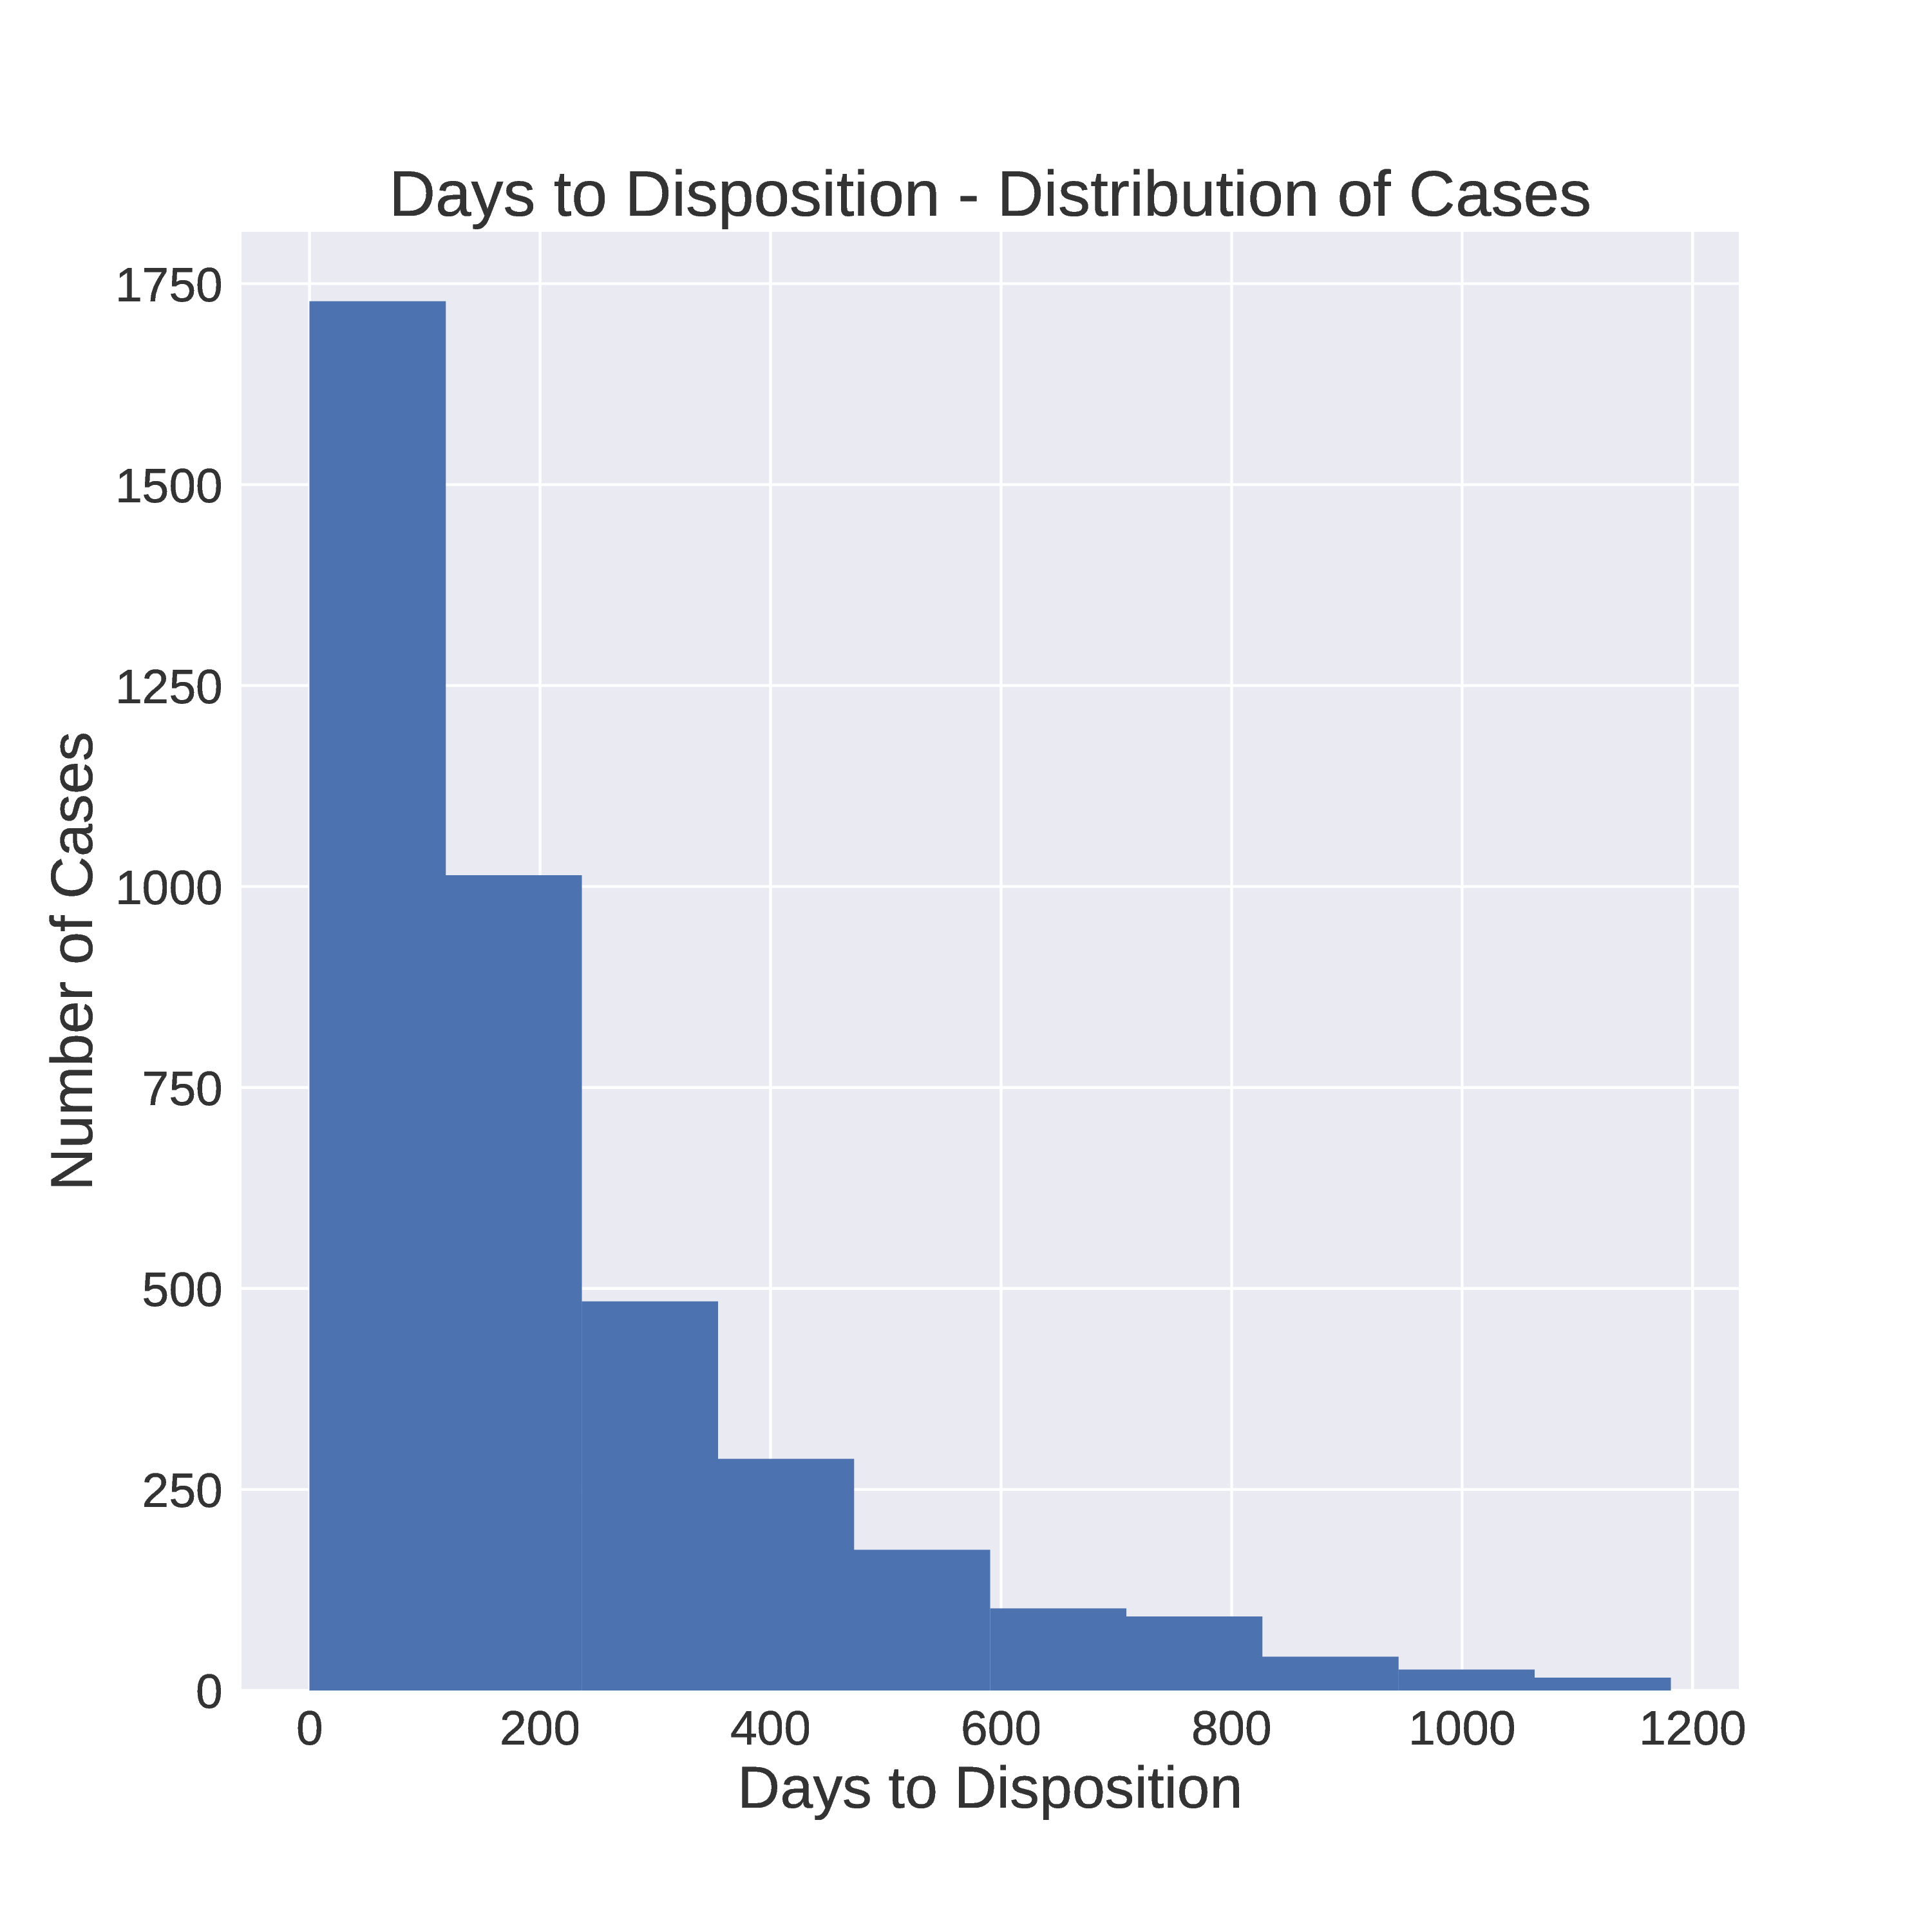
\includegraphics[width=0.70\columnwidth]{figures/time_to_dispo_histo/time_to_dispo_histo.png}
\caption{Histogram of the days it takes a case to reach disposition starting from the day the case is issued. 71 cases have negative time to disposition due to the case being re-issued in the course of the prosecutorial process. These cases have been dropped.
\label{fig:daysToDispo}%
}
\end{center}
\end{figure}

\begin{figure}[h!]
\begin{center}
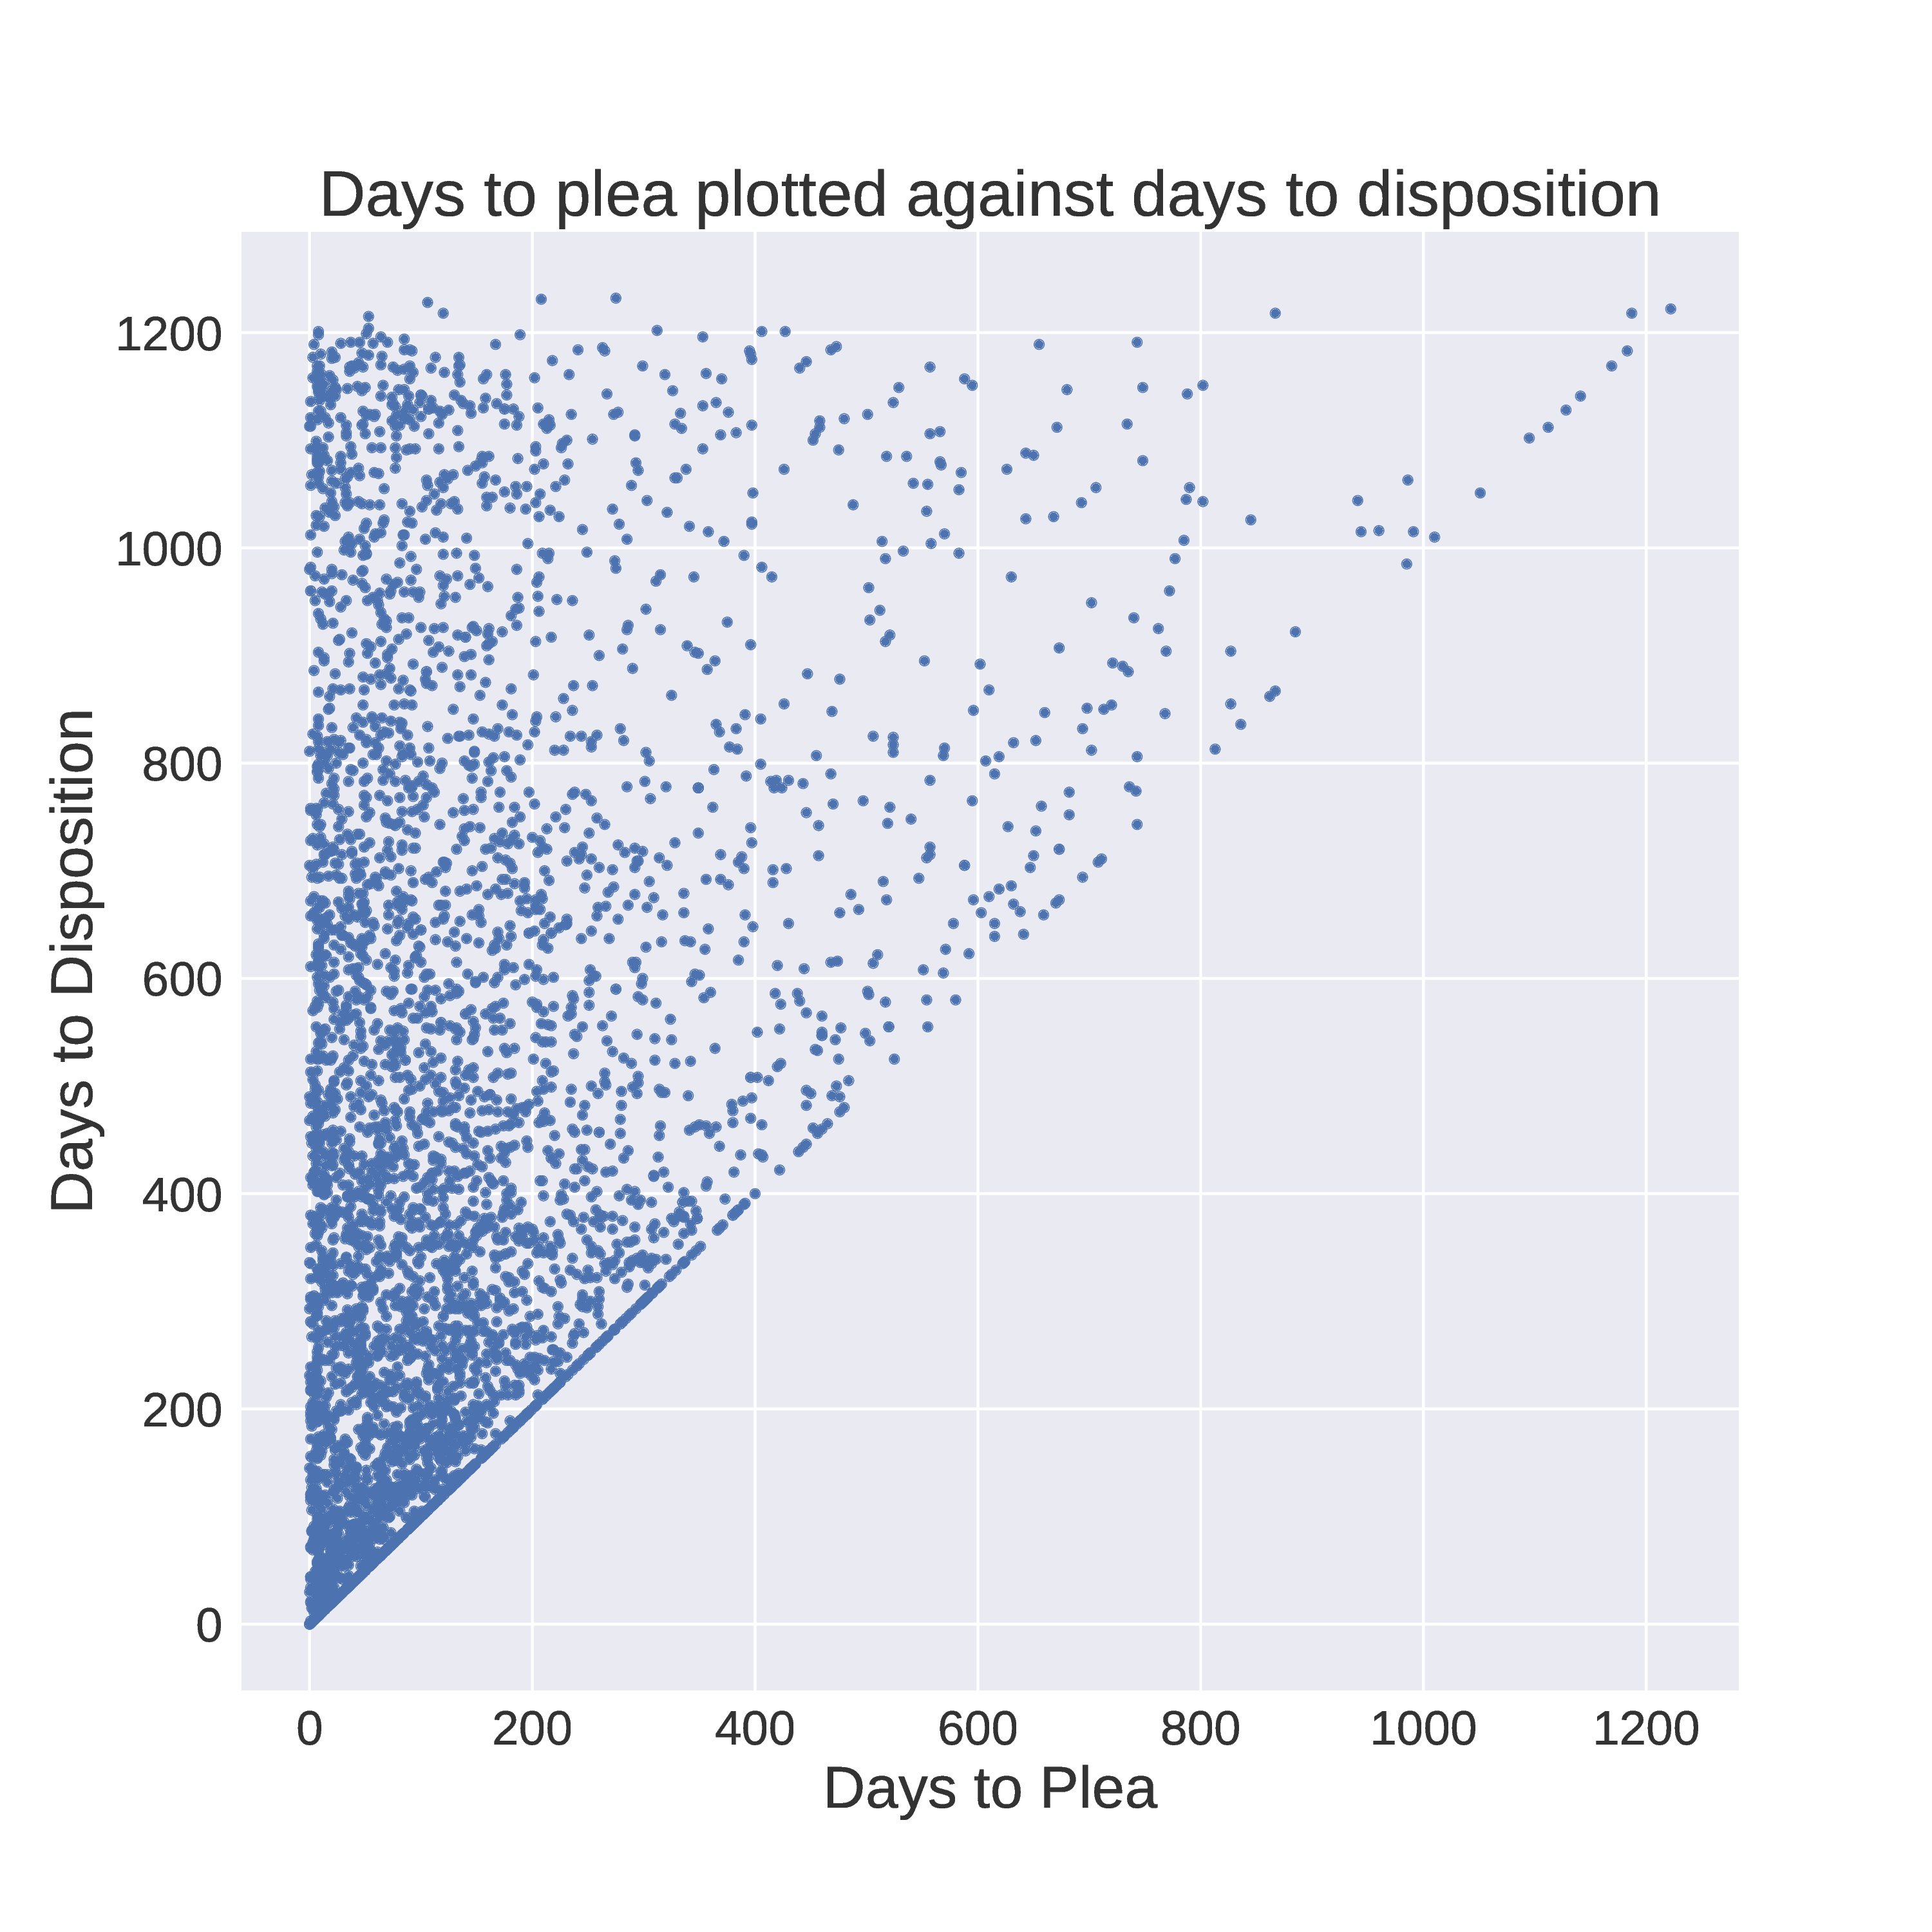
\includegraphics[width=0.70\columnwidth]{figures/plea_vs_disposition_scatter/plea_vs_disposition_scatter}
\caption{Days to plea plotted against days to disposition for felony cases issued by SCC in January-June 2014. No disposition can happen before the plea, hence the bottom right portion of the plot is empty. The SCC DA indicated the long duration of the prosecutorial process up to plea, which is uncharacteristically long due to peculiarities of the laws that in SCC do not require a defendant to enter a plea early in the case, would drive the long duration of the prosecutorial process to disposition. However, in this plot we see a large fraction of defendant-case pairs at the top left of the plot, with short time to plea, and yet long time-to-disposition, indicating that delays in entering a plea are only partially responsible for delays in the prosecutorial process up to disposition.
\label{fig:PleaVsDisposition}%
}
\end{center}
\end{figure}

To examine what other case factors might be the key drivers of delay
we look at case duration for cases with specific characteristics
independently. In \autoref{fig:Violins} we look at the distribution of
case duration (days-to-disposition) through multiple violin
plots. When the data can be split in a binary fashion, a violin plot
allows an intuitive comparison of the two distributions. The different
colors (blue and green) represent case-duration distributions for two
different subsets of the dataset. The distributions are normalized and
smoothed via kernel-density estimate with a Gaussian kernel. The
minimum and maximum values of each distribution reflect the shortest
and longest case in the dataset (and they need not be equal for the
two subsets).  We visualize the distributions of days-to-disposition
in this fashion for the following binary split of the data:
\begin{itemize}
\item gang enhancement \emph{vs} no gang enhancement on the charges,
\item single \emph{vs} multiple charges on the case,
\item single \emph{vs} multiple defendant,
\item guilty plea \emph{vs} any other plea,
\item no contest plea \emph{vs} any other plea,
\item not guilty \emph{vs} any other plea,
\item there was a preliminary hearing \emph{vs} no preliminary hearing on the case,
\item time waived \emph{vs}  time not waived,
\item trial \emph{vs} no trial.
\end{itemize}



More information of these features can be found in
\autoref{tab:Features}. We see that cases where the defendant
initially pleads guilty or no contest to charges are generally
resolved early in the process, while cases where the defendant pleads
not guilty have a flatter distribution, indicating more variability in
the prosecutorial process duration. Cases where the defendant pleads
not guilty are more likely to go to trial, so this is consistent with
what we see in the distribution of durations for cases that have
a preliminary hearing and/or a trial.  The presence of enhancements and
number of defendants are of specific interest as they had been clearly
identified by the SCC DA as possible key contributors to delays in the
prosecutorial process, but, while the first shows more power in the
tail, the presence of more than one defendant on a case or more than
one charge against a defendant do not, somewhat surprisingly, show
significant differences in case duration. However, we emphasize that
the number of cases with multiple defendants and multiple charges is
small, so this difference may not be statistically robust.



\begin{figure}[h!]
\begin{center}
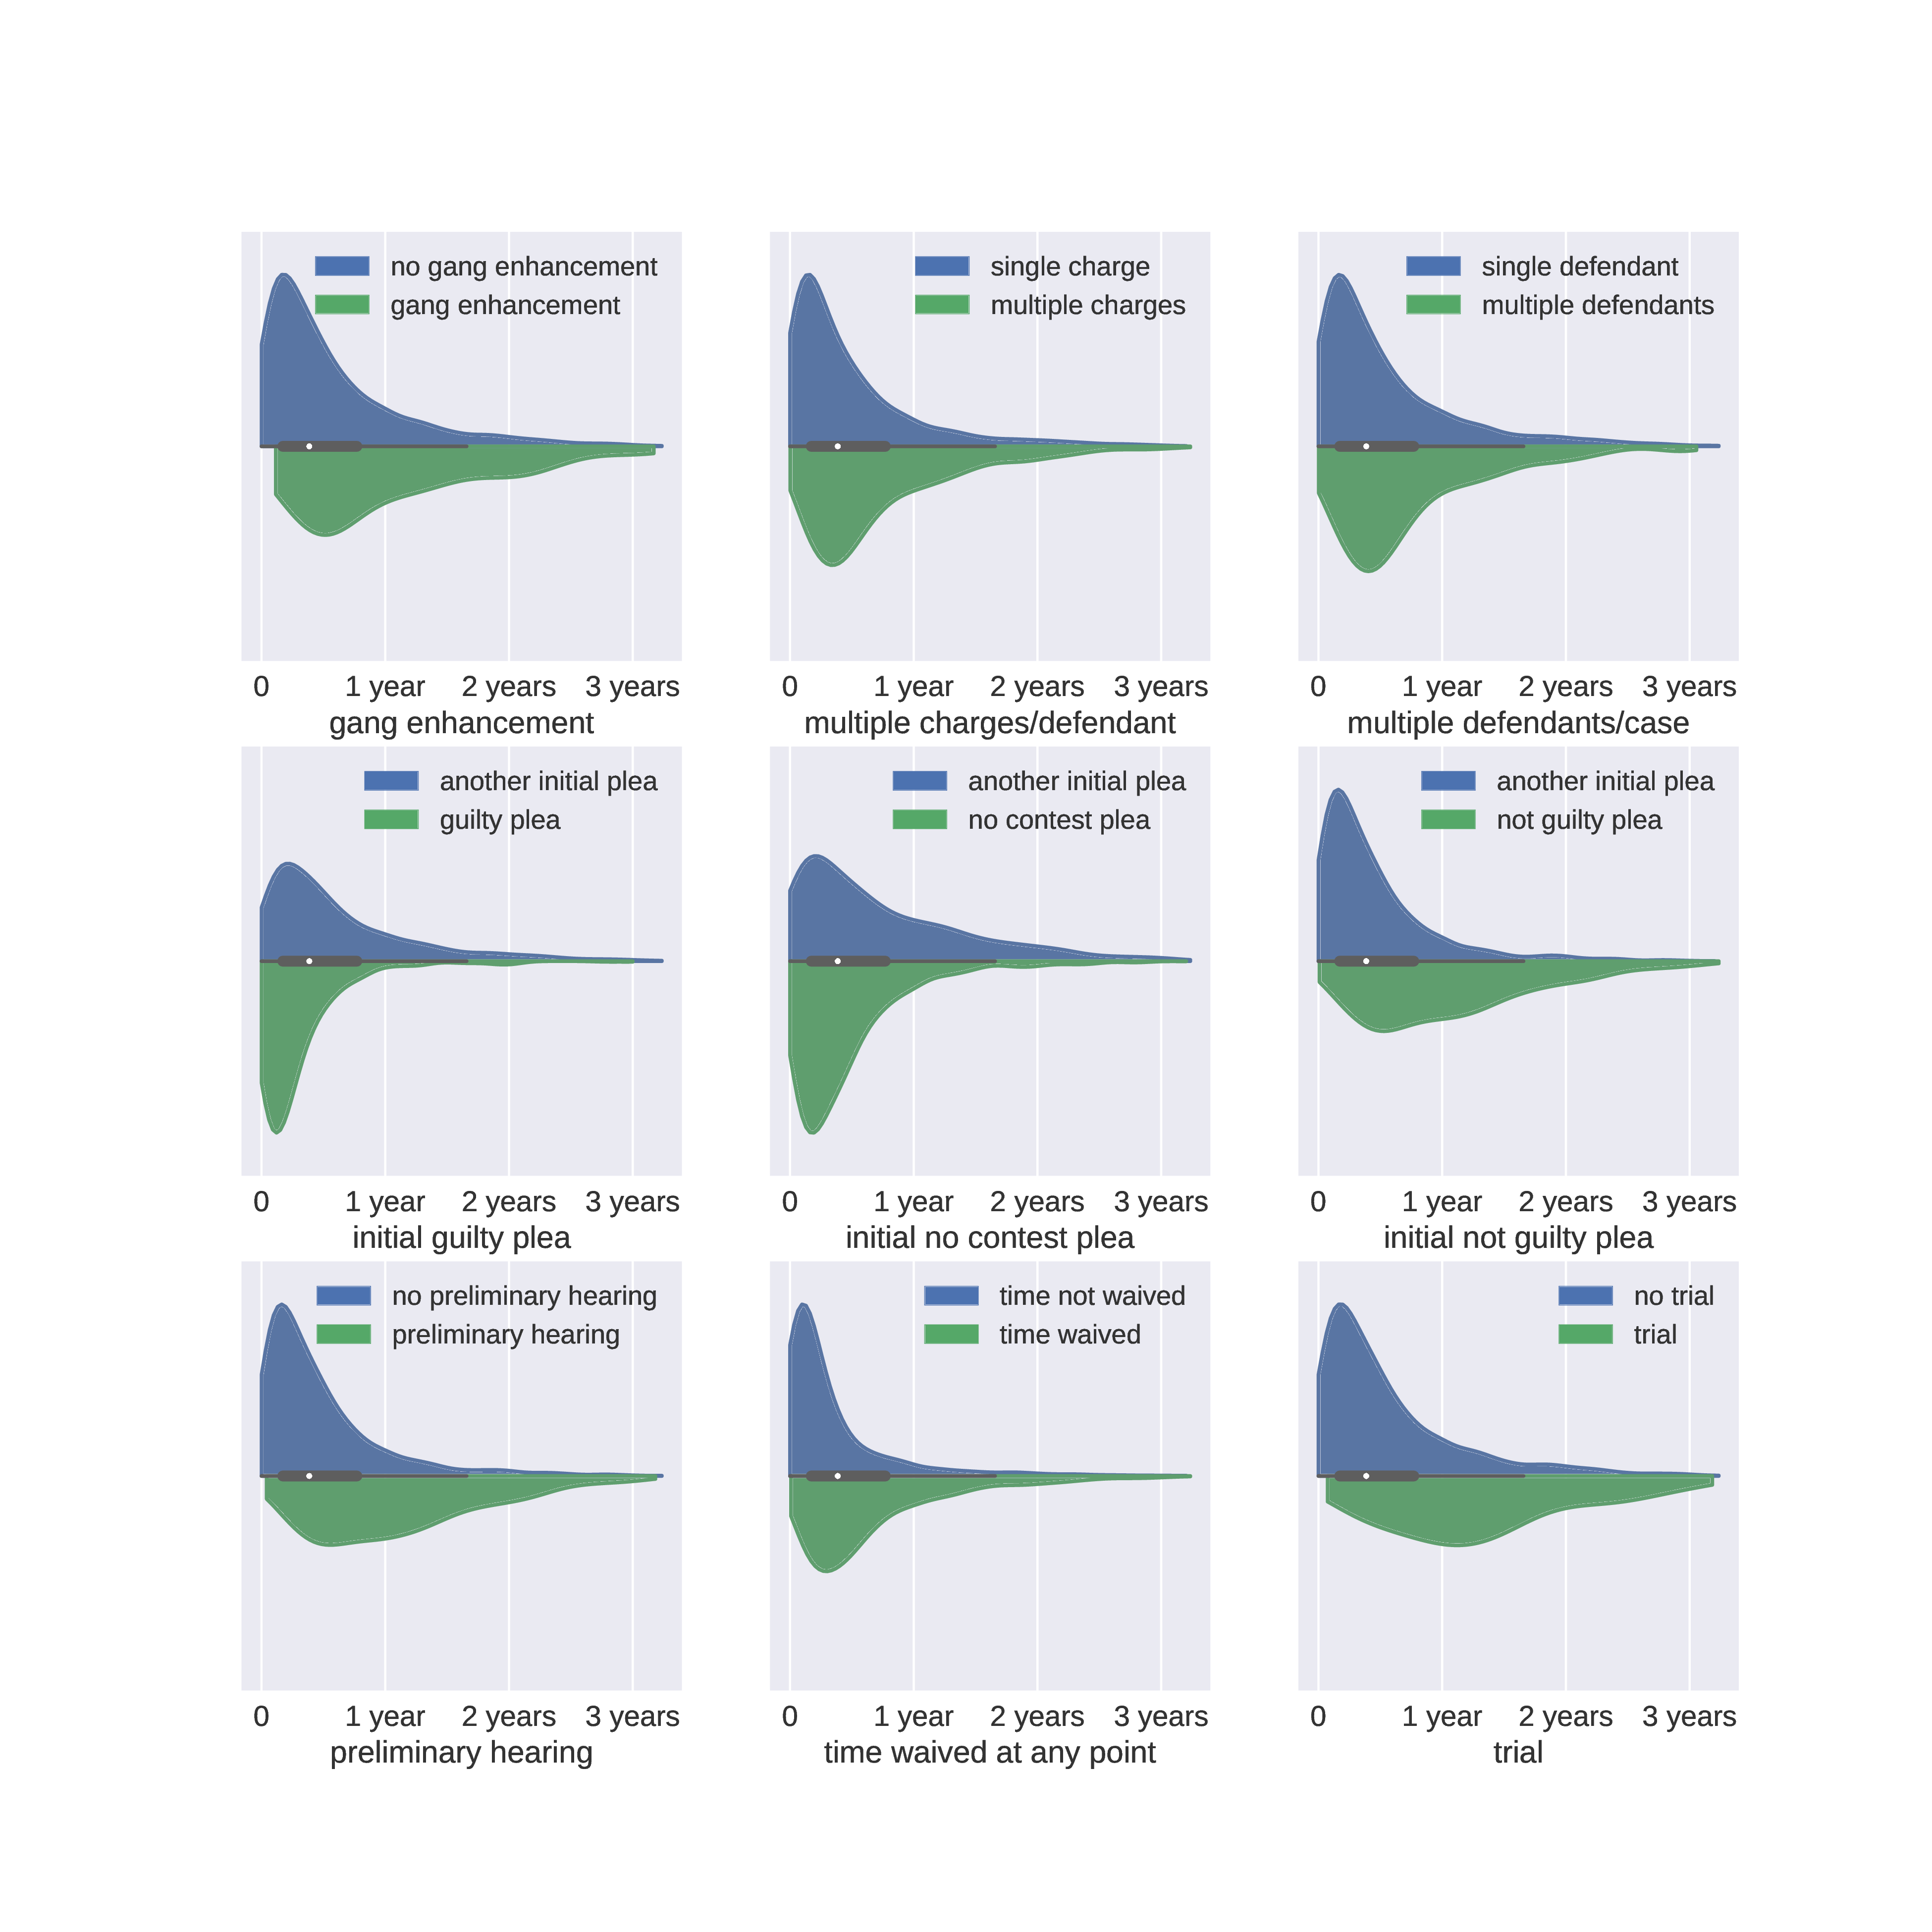
\includegraphics[width=0.70\columnwidth]{figures/multiple_violins4/multiple_violins4}
\caption{Distributions of duration of the full prosecutorial process, from case issuing to disposition, for felony cases issued between January and June 2014 by the SCC DA.  In each plot a distribution is shown as a histogram smoothed with a kernel density estimate for two samples (blue and green) split along the vertical axis for comparison: a so-called {\it violin} plot. Each violin plot shows the time-to-plea distribution for two subsets of our data. The horizontal bar indicates the IQR (thick bar), full statistical distribution without outliers (thin bar) and median (white dot) for the {\it top} distribution. We compare time-to-disposition for defendants (from the top left) going {\it vs} not going to trial, charged of crimes with {\it vs} without a gang enhancement, which plead guilty {\it vs} not guilty or {\it nolo contendere}, {\it nolo contendere} {\it vs} guilty or not guilty, charged with one {\it vs} more than one charge, who waived {\it vs} did not waive time (Table \ref{tab:Features}), who had {\it vs} did not have a preliminary hearing, charged as a single defendant {\it vs} with others (often occurring in gang related charges), and that pleas guilty {\it vs} not guilty or {\it nolo contendere}
\label{fig:Violins}%
}
\end{center}
\end{figure}

We can extend this examination to include other key events of a case. In Figure \ref{fig:ViolinsCustody}, we see time to arraignment, plea, disposition and the last event for defendants initially in custody against defendants initially not in custody. We see that both arraignment and plea most commonly happens very early in the process for those defendants initially in custody. Based on data from January through June of 2014 the median time to disposition for defendants in custody was 89 days. For those out of custody it was 192.5 days.

\begin{figure}[h!]
\begin{center}
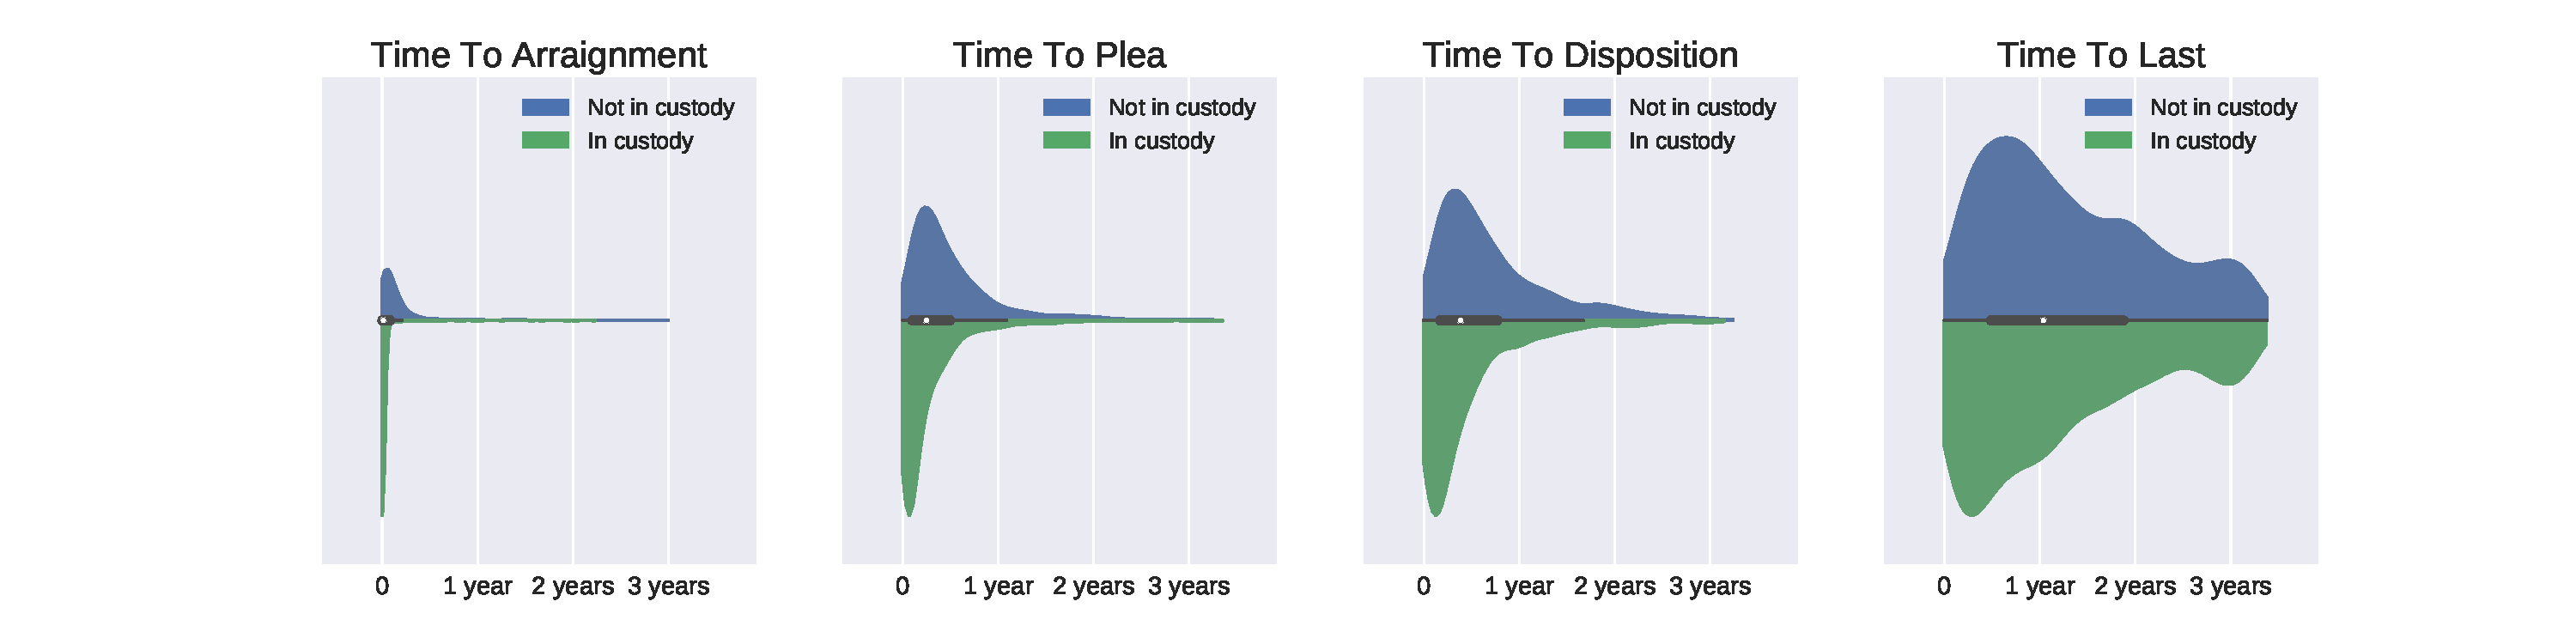
\includegraphics[width=0.70\columnwidth]{figures/4violins_custody/4violins_custody}
\caption{Duration of the prosecutorial process to disposition of cases for defendants initially in custody (blue) compared to defendants initially not in custody (green). No significant differences are observed. Details of the graphics are as in Figure \ref{fig:Violins}.
\label{fig:ViolinsCustody}%
}
\end{center}
\end{figure}

In \autoref{fig:ViolinsCompetency} we see the same breakdown for
defendants who have at some point during a case been found to be not
competent to stand trial plotted against all other defendants. While
this is a very rare occurrence,
%(MISSIN DATA) 
it drives the most significant difference in the distribution of
durations. The most common time of arraignment, plea, and disposition
for these defendants doesn't show significant differences, as the
motion to evaluate competence to stand trial would occur later in the
process.  However, the median duration to disposition extends past a
year, and most commonly the last event of these cases happens very
late in the process, after 1000 days. Based on data from January
through June 2014 the median time to disposition for defendants who
are at some point not competent to stand trial was 353 days. For other
defendants (excluding the aforementioned group) it was 135 days.



\begin{figure}[h!]
\begin{center}
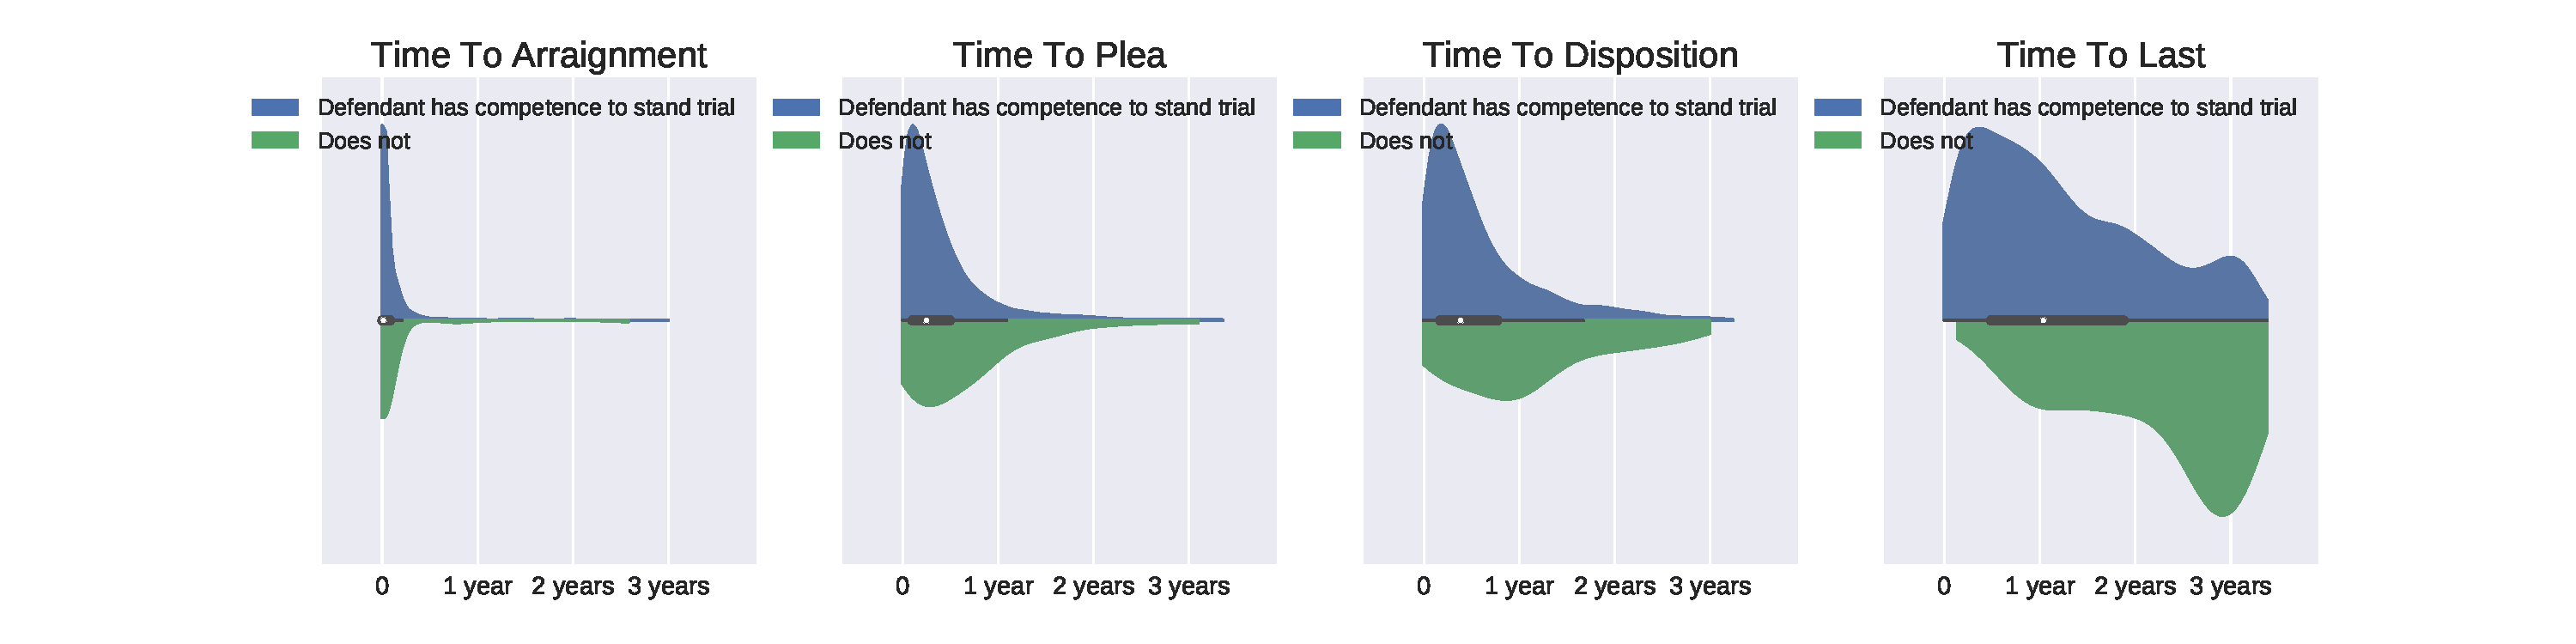
\includegraphics[width=0.70\columnwidth]{figures/4violins_pc1/4violins_pc1}
\caption{Duration of the prosecutorial process to disposition of cases for defendants initially in custody (blue) compared to defendants initially not in custody (green). Significant differences are observed, especially in the time-to-sentence, the distribution of which peaks later and has more power in the tail, and in the post-sentence duration, with an accumulation of defendant continuing to have court dates scheduled years after the beginning of the case. While these events occur after sentence and do not affect the primary metric we are testing (time-to-disposition and particularly when time-to-disposition extends past a year) it may affect the efficiency of the courts and cause delays in other cases. Details of the graphics are as in Figure \ref{fig:Violins}.
\label{fig:ViolinsCompetency}%
}
\end{center}
\end{figure}

Even though it takes more than twice as long to reach disposition for
defendants who have at some point been found to be not competent to
stand trial, this or any of the other engineered features will not
explain delays in the prosecutorial process on their own. The case of
being not competent to stand trial is an exception, applicable to 2\%
of the defendants in the dataset. In the last section of this paper,
we construct models to identify the most prominent drivers of
prosecutorial delay.


\subsection{Demographics}
Having information on age and race/ethnicity allows us to explore the demographics of the data. In Figure~\ref{fig:EthnicBreakdown} we see how the defendants's race/ethnicity breakdown compares to that of the population of SCC. There are some disparities between the two with some ethnicities over- or under- represented in the data. The defendants' age decreases steadily (Figure~\ref{fig:AgeBreakdown}) and the majority of defendants are male (Figure~\ref{fig:GenderBreakdown}). Greatest number of defendants come from the zipcodes around San Jose, as well as zipcodes 95037 and 95020 to the south of San Jose, see Figure \ref{fig:map}

\begin{figure}[h!]
\begin{center}
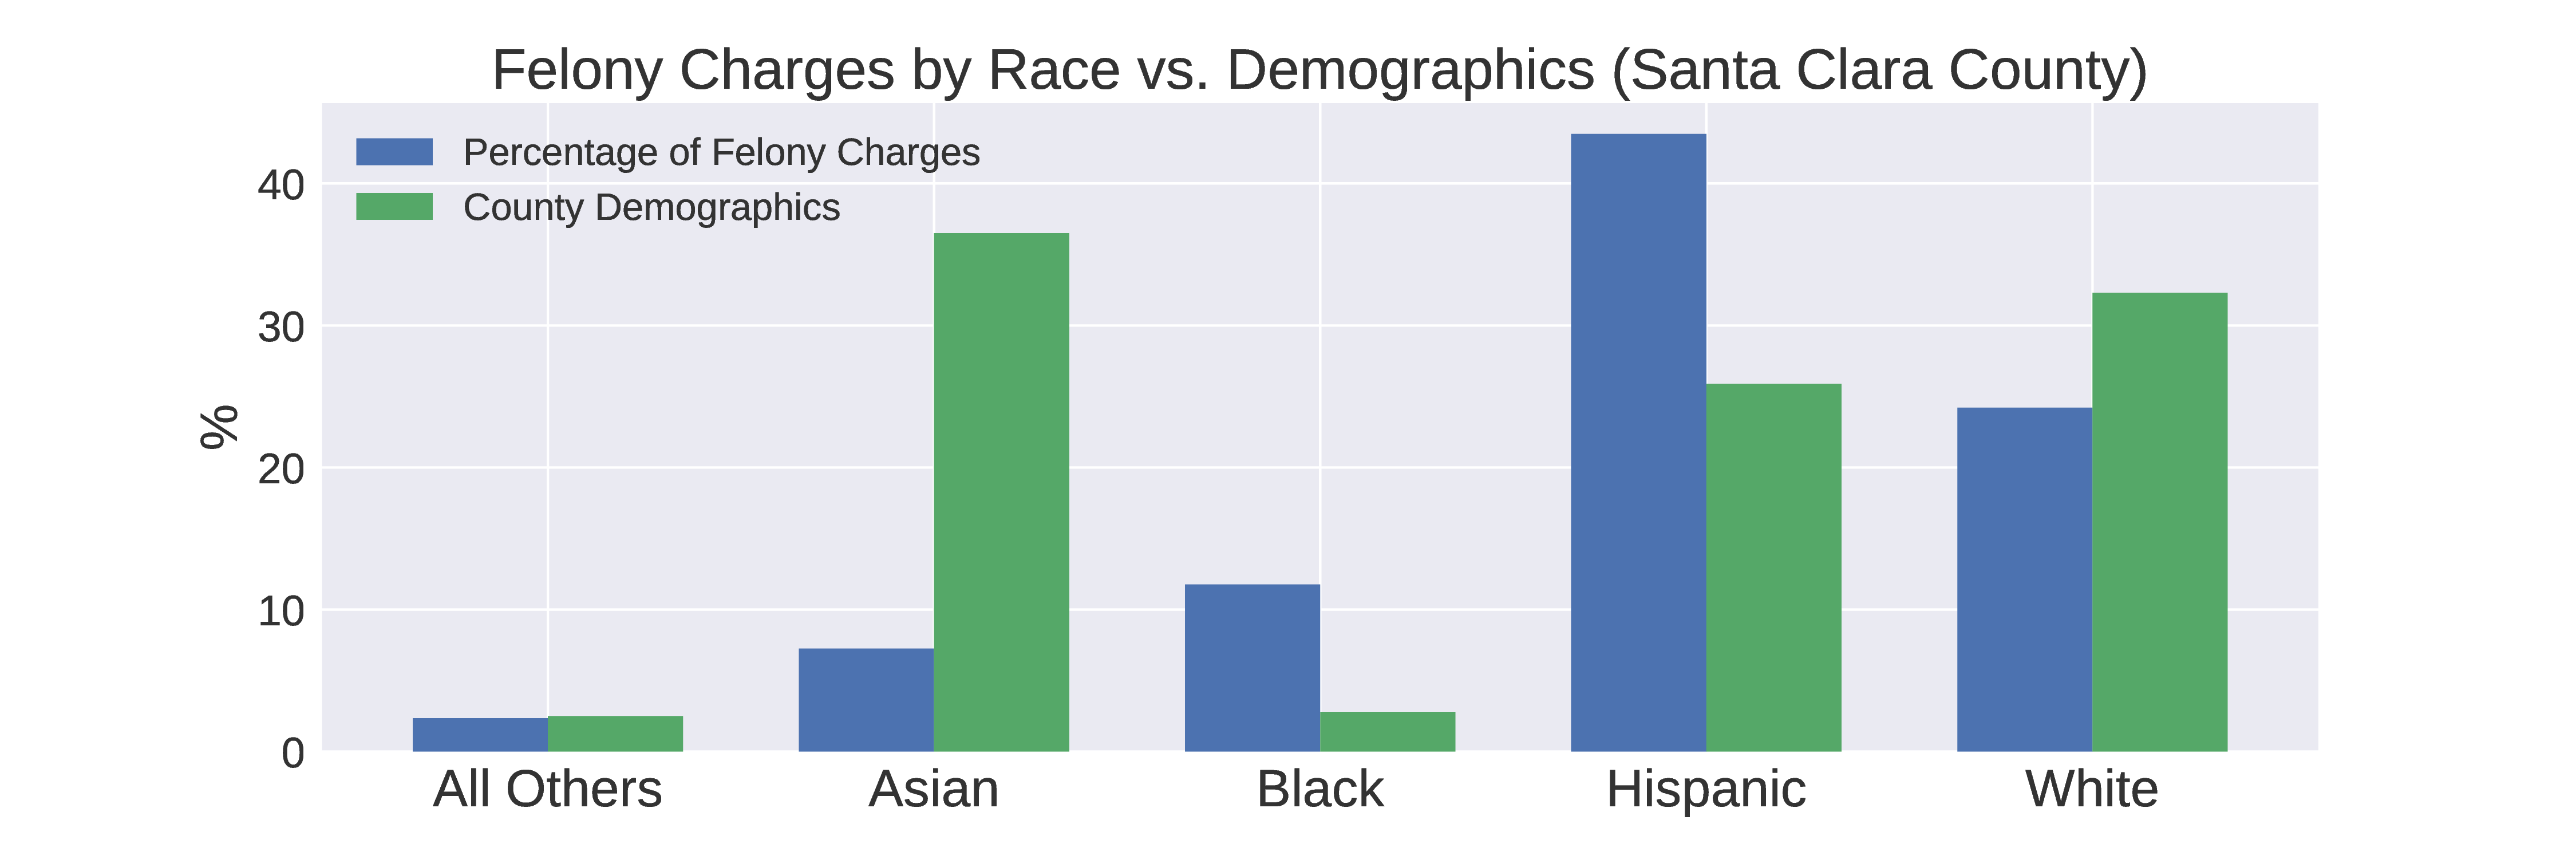
\includegraphics[width=0.70\columnwidth]{figures/chargesByRace_demographics1/chargesByRace_demographics1}
\caption{Ethnic breakdown of defendants in SCC felony cases issued between January and June of 2014 (blue) compared to the ethnic breakdown of the population of the county of Santa Clara (green).
\label{fig:EthnicBreakdown}%
}
\end{center}
\end{figure}

\begin{figure}[h!]
\begin{center}
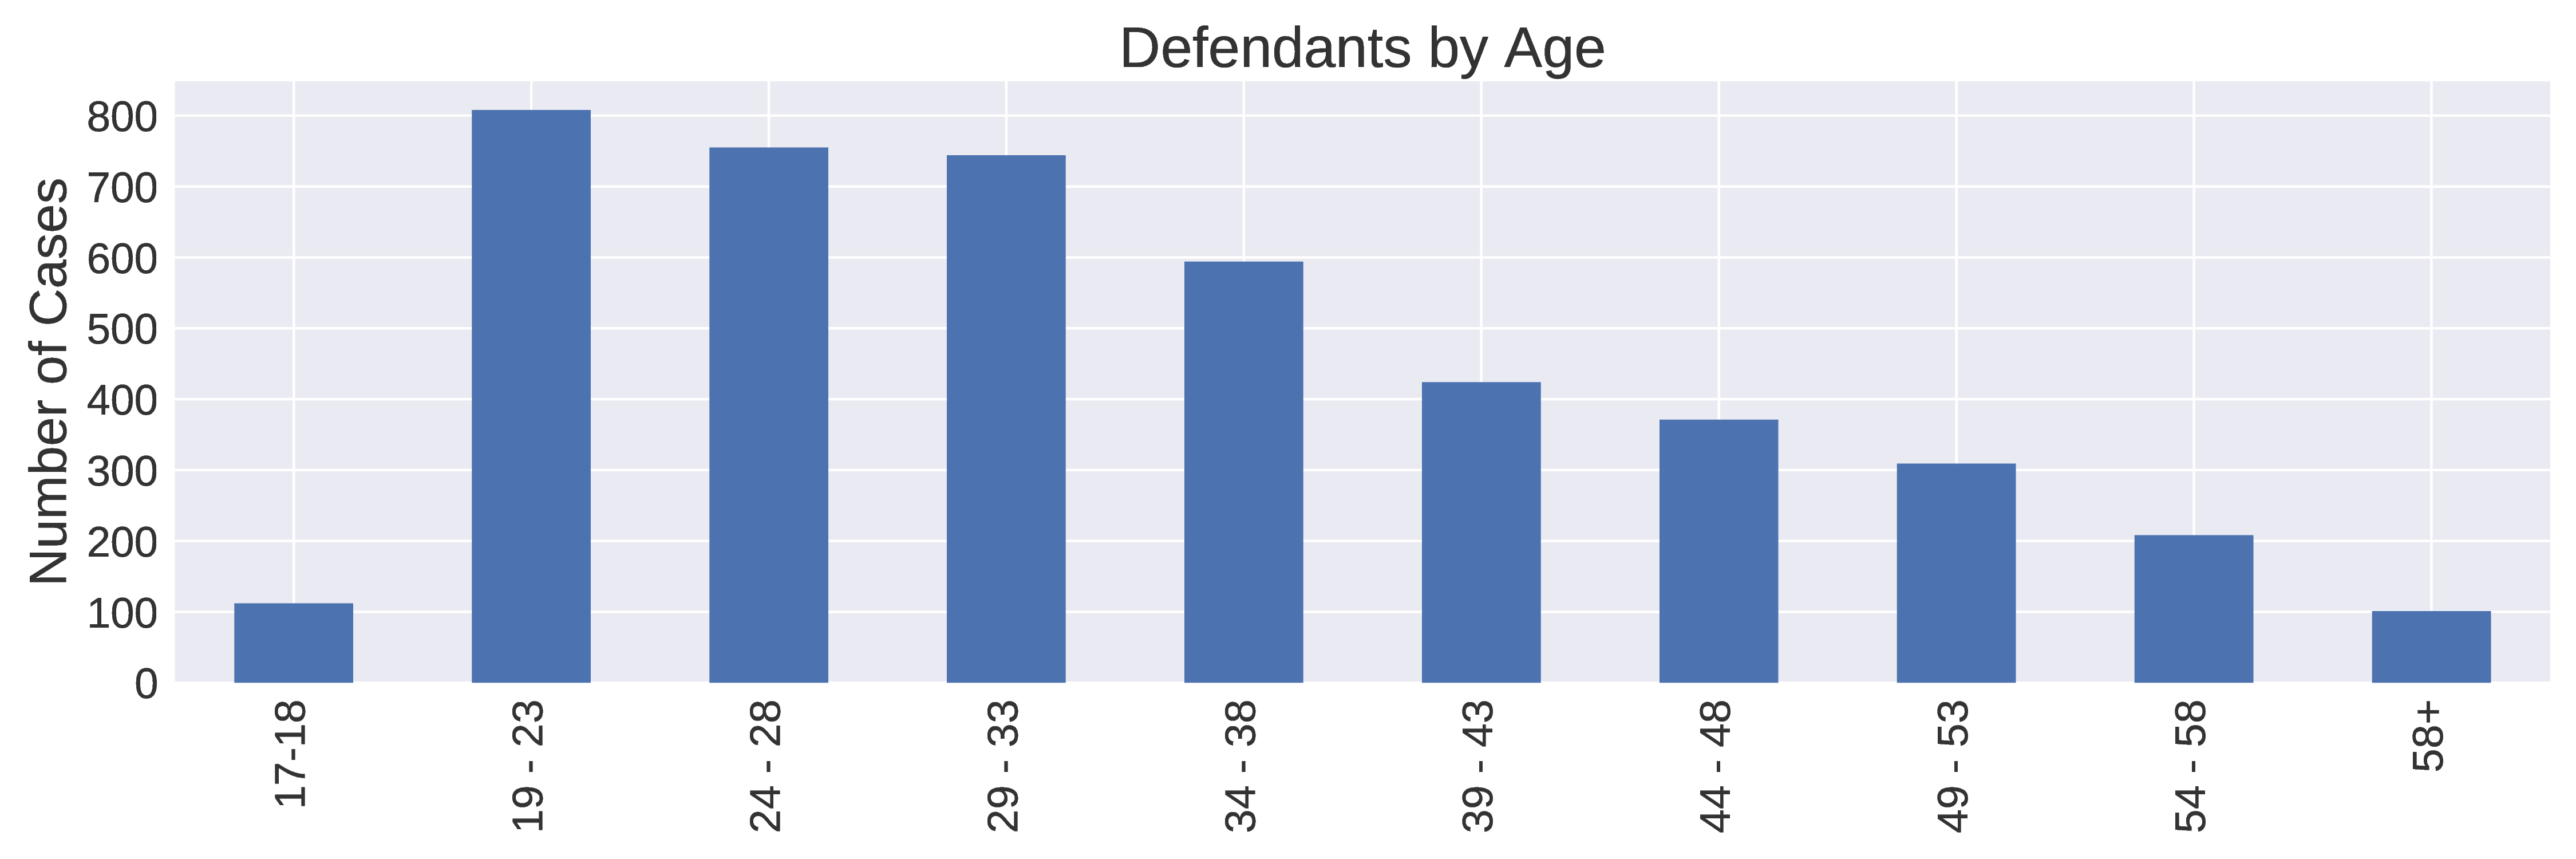
\includegraphics[width=0.70\columnwidth]{figures/age_histo/age_histo}
\caption{Age of defendants at crime commission in SCC felony cases issued between January and June of 2014 by 5 year age bins. Notice that the data only include defendants tried as adults.
\label{fig:AgeBreakdown}%
}
\end{center}
\end{figure}

\begin{figure}[h!]
\begin{center}
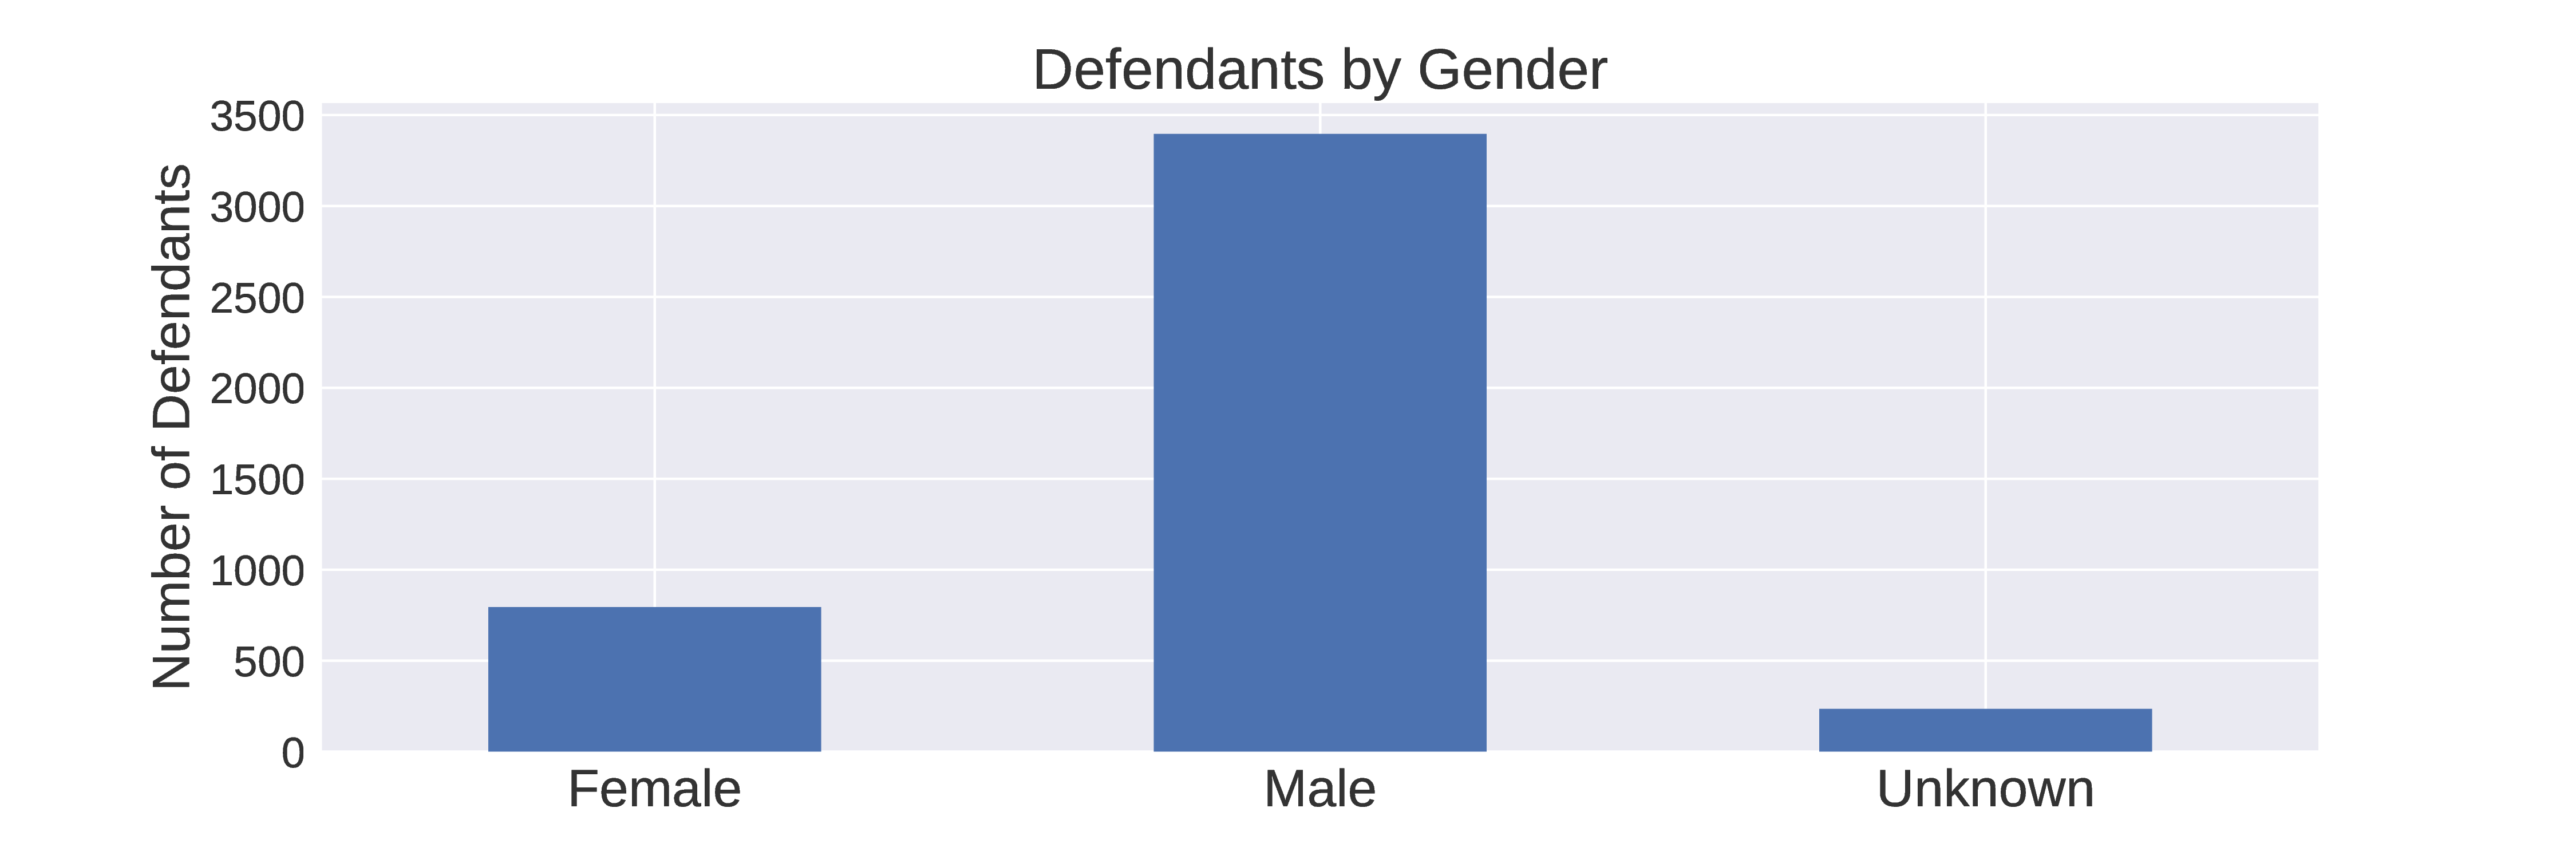
\includegraphics[width=0.70\columnwidth]{figures/gender/gender}
\caption{Gender of defendants in SCC felony cases issued between January and June of 2014. 77\% of the defendants identified as males, 18\% as females, and the gender is unknown for 5\%.
\label{fig:GenderBreakdown}%
}
\end{center}
\end{figure}

\begin{figure}[h!]
\begin{center}
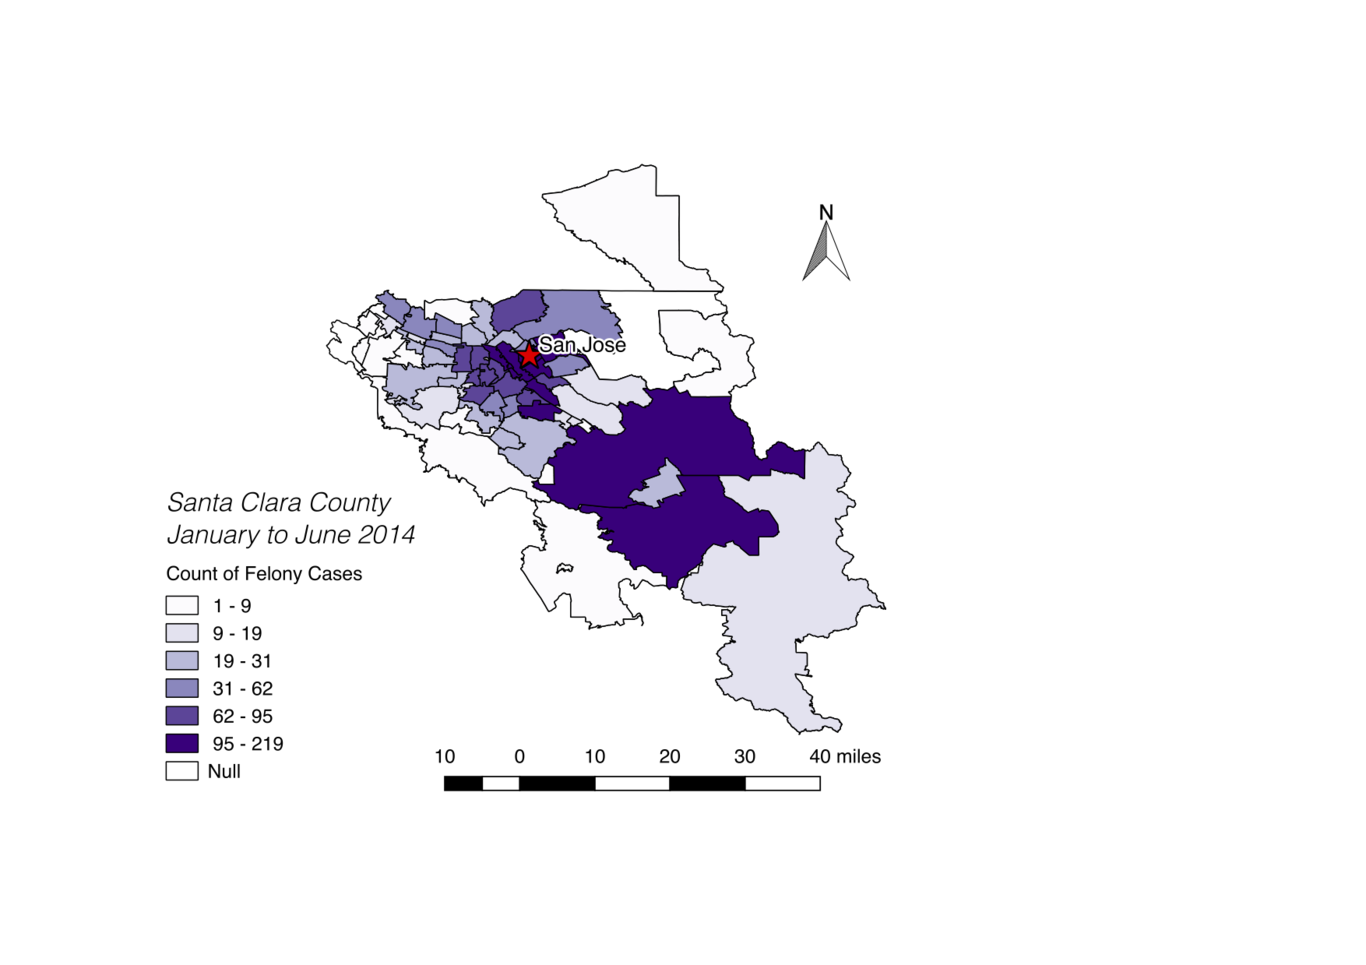
\includegraphics[width=0.70\columnwidth]{figures/scc_map1/scc_map1}
\caption{Number of defendants by zipcode of residence. Most commonly defendants live in the areas in and around San Jose. Zipcodes 95037 and 95020 to the south of San Jose are also prominently featured.
\label{fig:map}%
}
\end{center}
\end{figure}

Using the demographics of the data and the timeline of cases gives us an
access to case duration for different demographics. In Figure
\ref{fig:DurationsEthnicity} we see case duration by race/ethnicity.
Duration is measured in days between the creation of a case until its
resolution. From this figure, we can conclude that there is no
statistically significant difference in the duration of the process for
different races/ethnicities in our case dataset.

\begin{figure}[h!]
\begin{center}
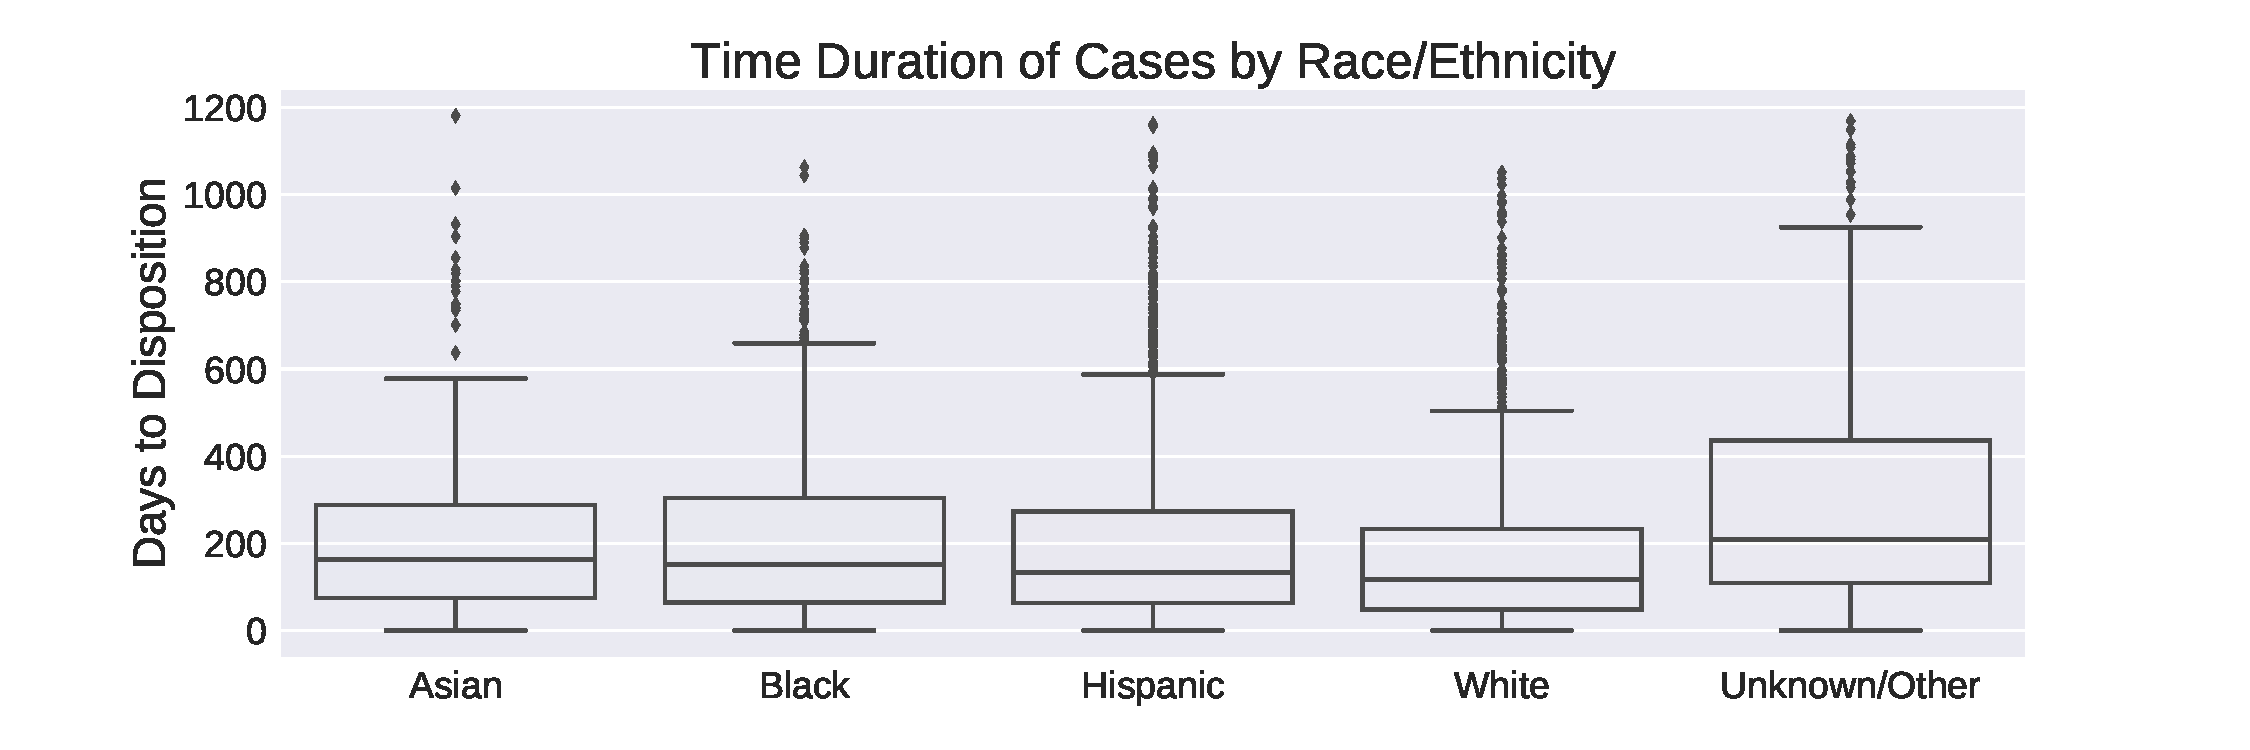
\includegraphics[width=0.70\columnwidth]{figures/race_boxplot/race_boxplot}
\caption{Case duration, measured as days between case issue and disposition, by different race/ethnicitiy. For each ethnic group, the horizontal line within the box represents the median case duration. The box represents the interquartile range (IQR), the "whiskers" represent the full distribution, excluding statistical outliers, which are shown as individual data points. No statistically robust differences appear, as all the medians fall in the 25--75 percentiles of all other groups. Curiously, the distribution for Unknown/Other (missing and uncommon ethnic groups) is only marginally consistent with most of the other distributions. We speculate this may be due to cases issued against defendants that are not in custody and not reachable/fleeing from custody, and wish to test this in the future
\label{fig:DurationsEthnicity}%
}
\end{center}
\end{figure}

In Figure \ref{fig:DurationsMeth}~we have isolated the most commonly
found charge in the data, violation of Health and Safety Code 11377(a)
which is the possession of methamphetamine. The figure shows case
duration for different races/ethnicities on the same charge. Again, we
conclude that there is no statistically significant difference in the
duration of the process for different races/ethnicities.

\begin{figure}[h!]
\begin{center}
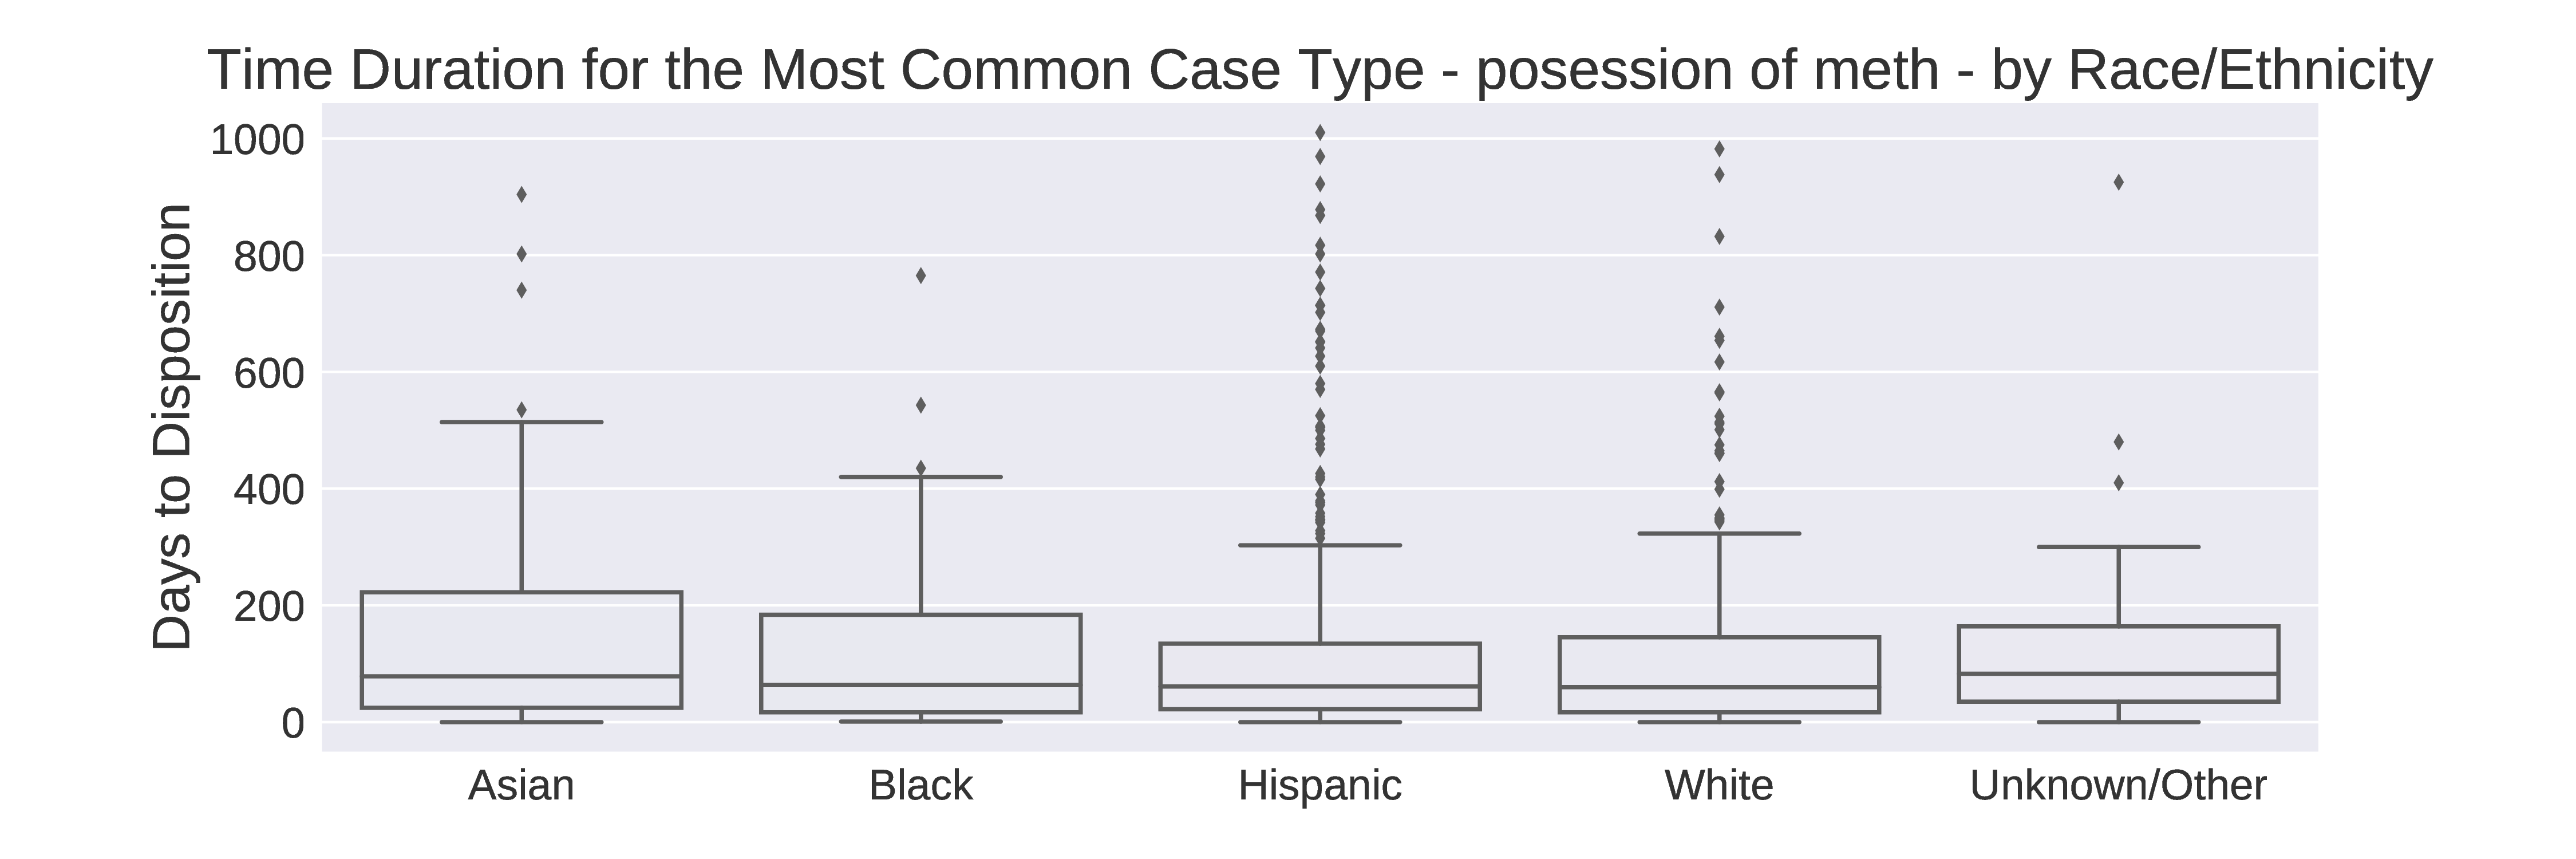
\includegraphics[width=0.70\columnwidth]{figures/race_modalcrime_boxplot/boxplot_race_modalcrime}
\caption{As in Figure \ref{fig:DurationsEthnicity}: prosecutorial process duration by ethnicity/race for the most common charge issued by the SCC's DA in January through June of 2014, HS 11377(a) -- possession of methamphetamine -- to correct for compounding biases in crime by race (e.g. frequency of crime by ethic group). As for the full charges sample, the distribution of prosecutorial duration is consistent for all ethnic groups.
\label{fig:DurationsMeth}%
}
\end{center}
\end{figure}

Lastly, in \autoref{fig:2ndModal} we have isolated the second most
common charge found in the dataset, theft of property---PC 459-460(b)--
since Proposition 47 reclassified HS 11377(a) and this would no longer
be a felony in charges issued after 2014. There are only 312
observations of this kind, but again, no differences appear.


\begin{figure}[h!]
\begin{center}
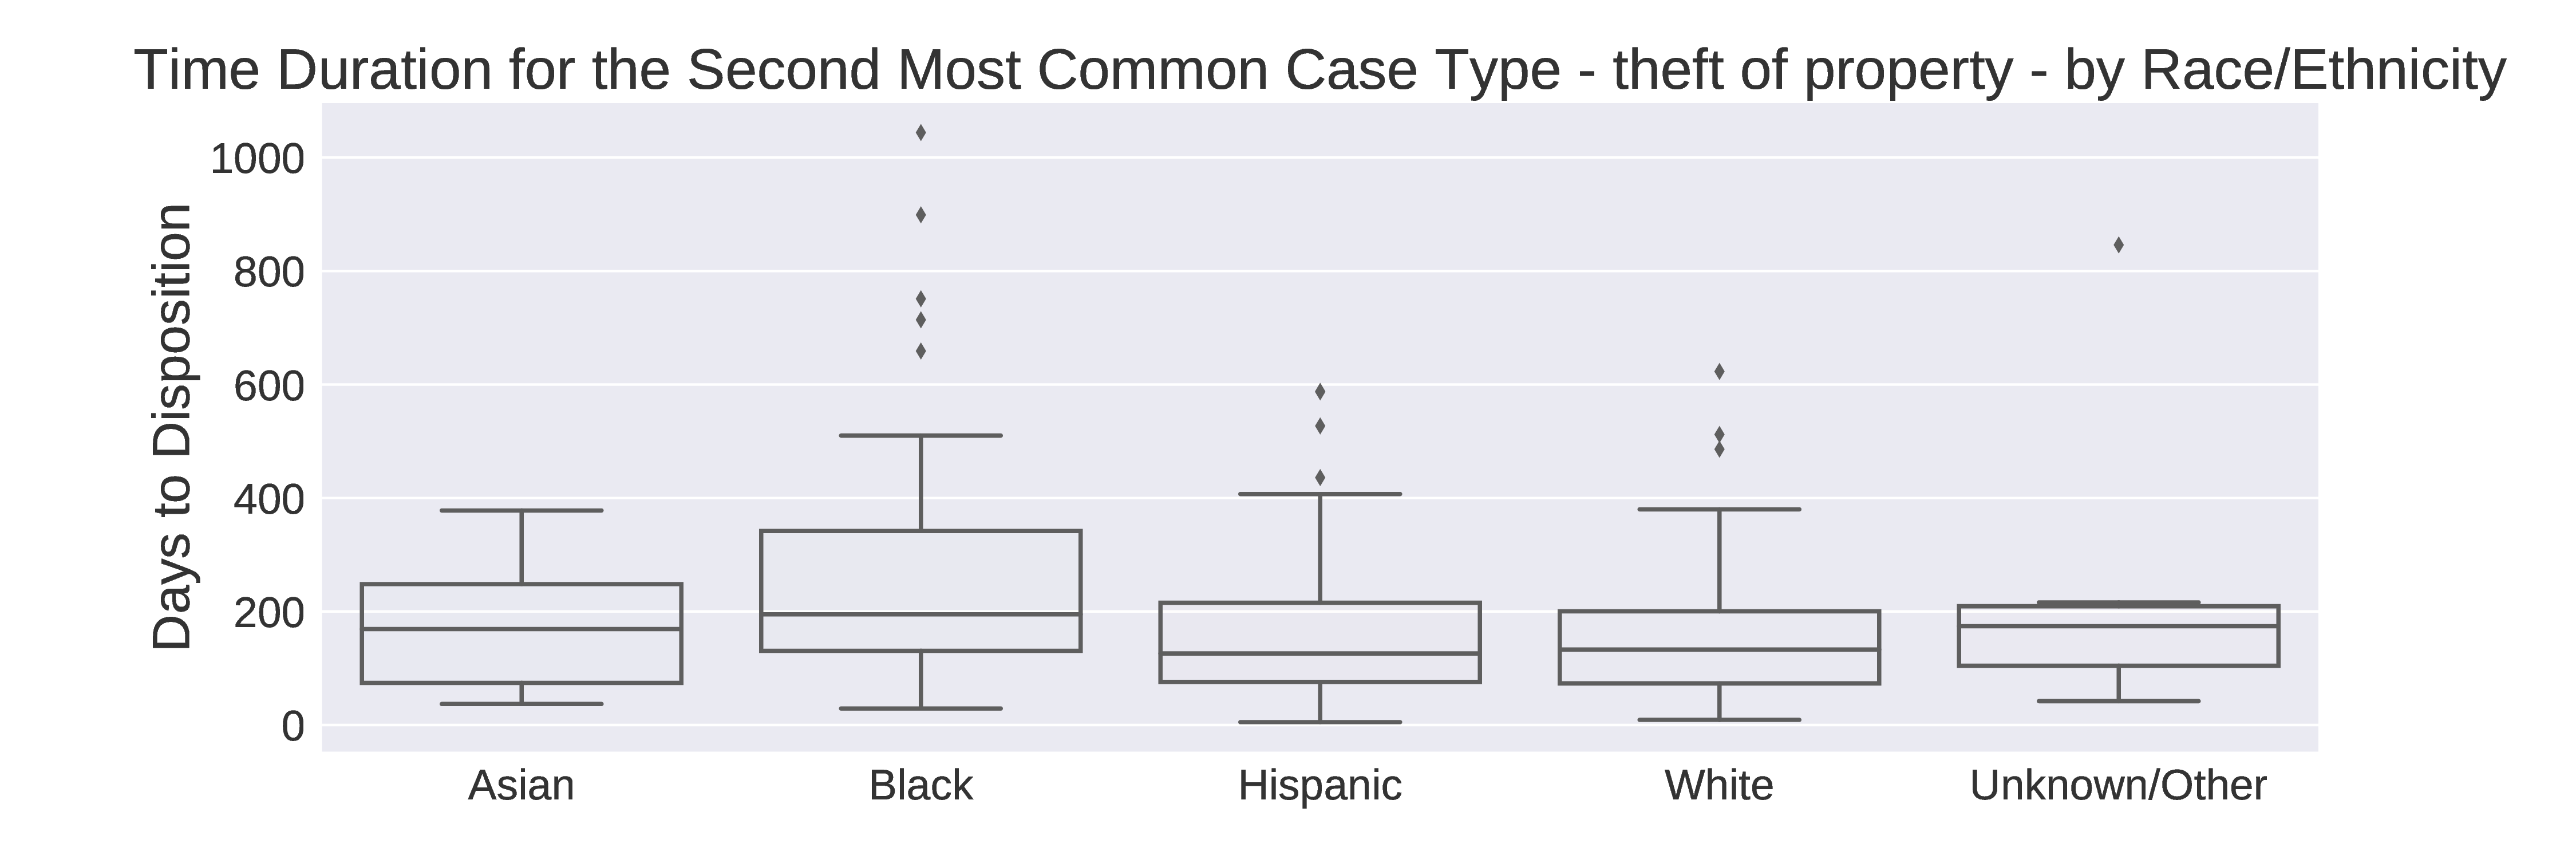
\includegraphics[width=0.70\columnwidth]{figures/boxplot_race_2ndmodalcrime/boxplot_race_2ndmodalcrime}
\caption{As in Figure \ref{fig:DurationsEthnicity}: prosecutorial process duration by ethnicity/race for the second most common charge issued by the SCC's DA in January through June of 2014, PC 459-460(b) -- theft of property. As for the full charges sample, the distribution of prosecutorial duration is consistent for all ethnic groups.
\label{fig:2ndModal}%
}
\end{center}
\end{figure}

\section{Visual analysis tools}\label{visual-analysis-tools}

\subsection{Visual tool to enable data exploration}

While we will perform a statistical analysis of the data, this work
will be generated from a typical data-science approach: finding,
comprehending, merging, and sorting data; and applying statistical
tools and other filters to identify trends in the data. These are not
tasks that are suited for a DA's office, which generally has little
training for this purpose, and has many other important legal tasks to
perform. Therefore, it is desirable to automate much of this process
and provide a means for the prosecutors to engage with their data so
that they can identify trends without advanced data skills.

Even before the final SCC dataset was in our hands, we generated
concepts for the visualization using synthetic datasets. These
datasets were constructed with a small set of features that we
expected would be of interest to the attorneys. This includes the
durations of four phases of prosecution, race and gender, and
age. Although these are only some of the important variables to
consider in our visualization and modeling activities, we chose these
for development purposes so that we could determine how best to handle
arbitrary variables we may want to display. In particular, we have
been able to prototype the ability to filter our data based on binary,
categorical, and continuous variables. All of the engineered features
are enabled in the final version of the dashboard, and new variables
can be easily added on as needed.

The simplest form of this visualization is a stacked horizontal bar
plot (\autoref{fig:sshot}). Each bar represents a category of
comparison that is selected by the user, (e.g., race/ethnicity, age
group, or court category referring to the court of
disposition). Visual comparisons are made via three information
channels for each bar: its location on the $x$-axis, width, and color.

The location of the bar encodes the time for a given phase to commence
relative to the start of some other chosen phase. Location attributes
are most easily compared by a user when they are placed on the same
scale \hyperref[csl:13]{(Munzner 2014}; \hyperref[csl:14]{Wilkinson
  2005)}. Therefore, we provide the ability to choose which phase to
compare against and align the $x$-axis (time) such that the phase
begins at time $t = 0$, and earlier phases are displayed on the
negative portion of the scale. For overall case-duration comparison,
we align to the beginning of the first phase, where the start of each
case is displayed at $t = 0$.


\begin{figure}[h!]
\begin{center}
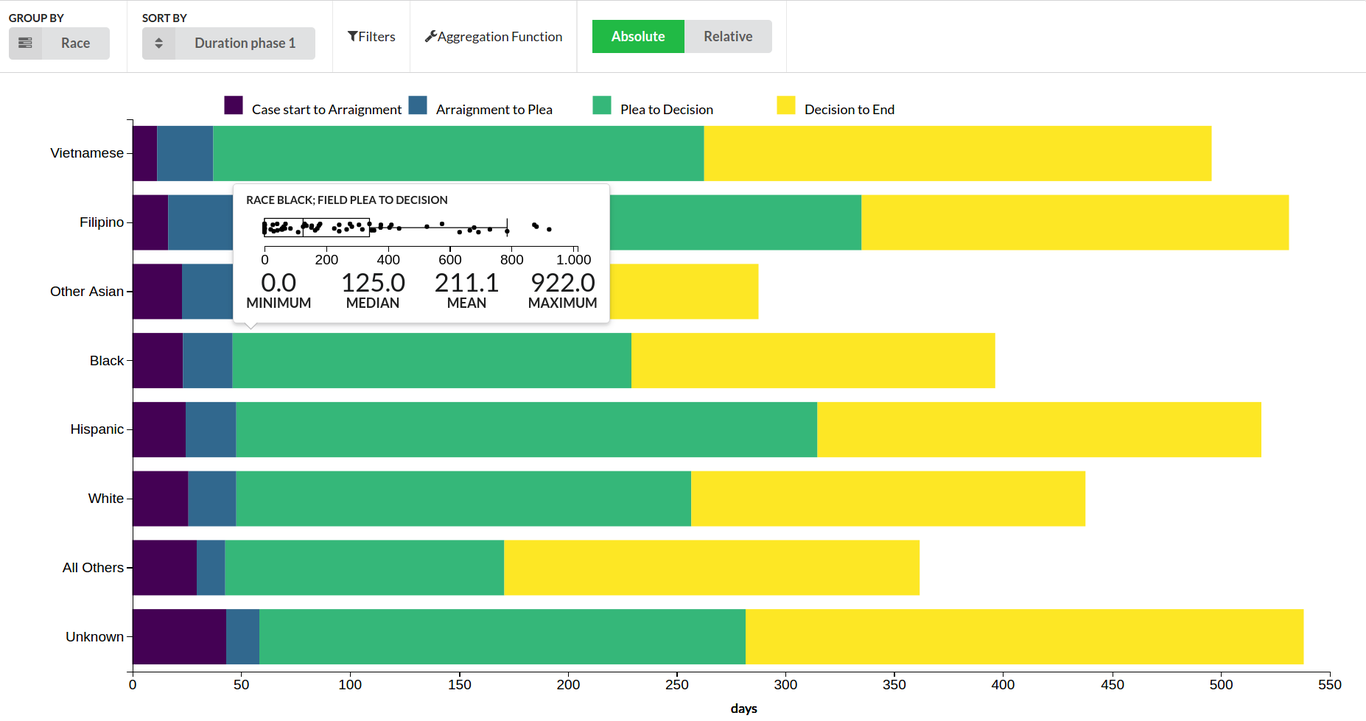
\includegraphics[width=0.70\columnwidth]{figures/sshot_original_original/sshot}
\caption{Screenshot of our visualization tool designed to enable exploration of SCC prosecutorial data running in the Chrome web browser. The visualization tool breaks down the prosecutorial process into four phases: case issue-to-arraignment, arraignment-to-plea, plea-to-disposition, disposition-to-last logged event, and enables aggregation, filtering, and sorting on other axes: demographic, court related categories, etc. Here the visualization is using synthetic data, binned and aggregated on age ranges and sorted by the duration of the second phase (``arraignment to plea''). Note that the $x$-axis (days) is aligned such that the second phase starts at $t = 0$ and the first phase is shown extending in to the negative portion of the domain. Also shown is an example of the distribution information that is displayed when the user hovers over a bar using a pointing device: minimum, maximum, and a box plot showing the entire distribution for that prosecutorial phase (arraignment-to-plea) and the category belonging to that bar (defendant between 21 and 25 years of age).
\label{fig:sshot}%
}
\end{center}
\end{figure}

The width of the bar encodes the duration of each phase. These values are calculated as the difference of the times from the beginning of each case to the ends of two consecutive phases. Since these times are determined by our own categorization scheme for the case events, the phase durations will be subject to some error depending on how well we can identify the demarcations between the phases in the data and how well the data is entered into the DA's case management system.

The color of the bars encode which of the four phases is being represented. We use four colors drawn widely and uniformly from the viridis color palette \hyperref[csl:3]{(van der Walt and Smith 2015)}. The colormap was developed for the Matplotlib python graphics package and is now its default color palette as of version 2.0. Viridis has two desirable properties: it is perceptually uniform (meaning that the scale is uniformly smooth and does not induce a perception of structure) and robust to common forms of colorblindness. These colors are easily distinguishable.

An additional channel of information is available when hovering the mouse pointer over any aggregated bar, showing a one-dimensional horizontal scatterplot of the underlying data along a time axis. Also displayed is a boxplot of the distribution, as well as the elementary statistics of minimum, maximum and median.

A prototype of this dashboard using synthetic data is available at \href{http://bit.ly/2hbPqrL}{http://bit.ly/2hbPqrL}.

\section{Modeling and Feature Importance}

Binary classifiers take the values of the input features $x_{i}$ and output $y_{i} \in \{0,1\}$. Decision trees do this by partitioning the feature space into subspaces, such that the divisions give rise to final regions with learned classifications. The subspaces divided at each step of the construction of the tree represent nodes of the tree, and the final set of subspaces after the desired number of partitions are created are the tree's terminal leaves.

These partitions can be complex, with many splits, leading to many nodes with high accuracy (the so-called ``purity'' of the leaves, determined by various measures). These trees are ``strong'' learners, but generally exhibit poor performance on unseen data in high dimensions since they are overfit on training data. Conversely, the partitions can be simple, with few splits (possibly even only one) having nodes with lower purity. These trees are called ``weak'' learners, but have the advantage of being simple and not overfitting the training data.

Robust against outliers and data transformations, decision trees are fast and their results are interpretable. In isolation, decision trees can perform well and have low bias, but they tend to exhibit high variance as errors in the first node quickly propogate through the children nodes of the tree when applied to data unseen by the model \hyperref[csl:4]{(James et al. 2013)}. In order to reduce this variance, ensemble methods are frequently employed. We attempt to improve the performance of our models using two such techniques: Random Forest and Gradient Boosted Decision Trees. Both models are implemented in Python using packages scikit-learn \hyperref[csl:5]{(Pedregosa et al. 2011)} and xgboost \hyperref[csl:6]{(Chen and Guestrin 2016)}.

\begin{figure}[h!]
\begin{center}
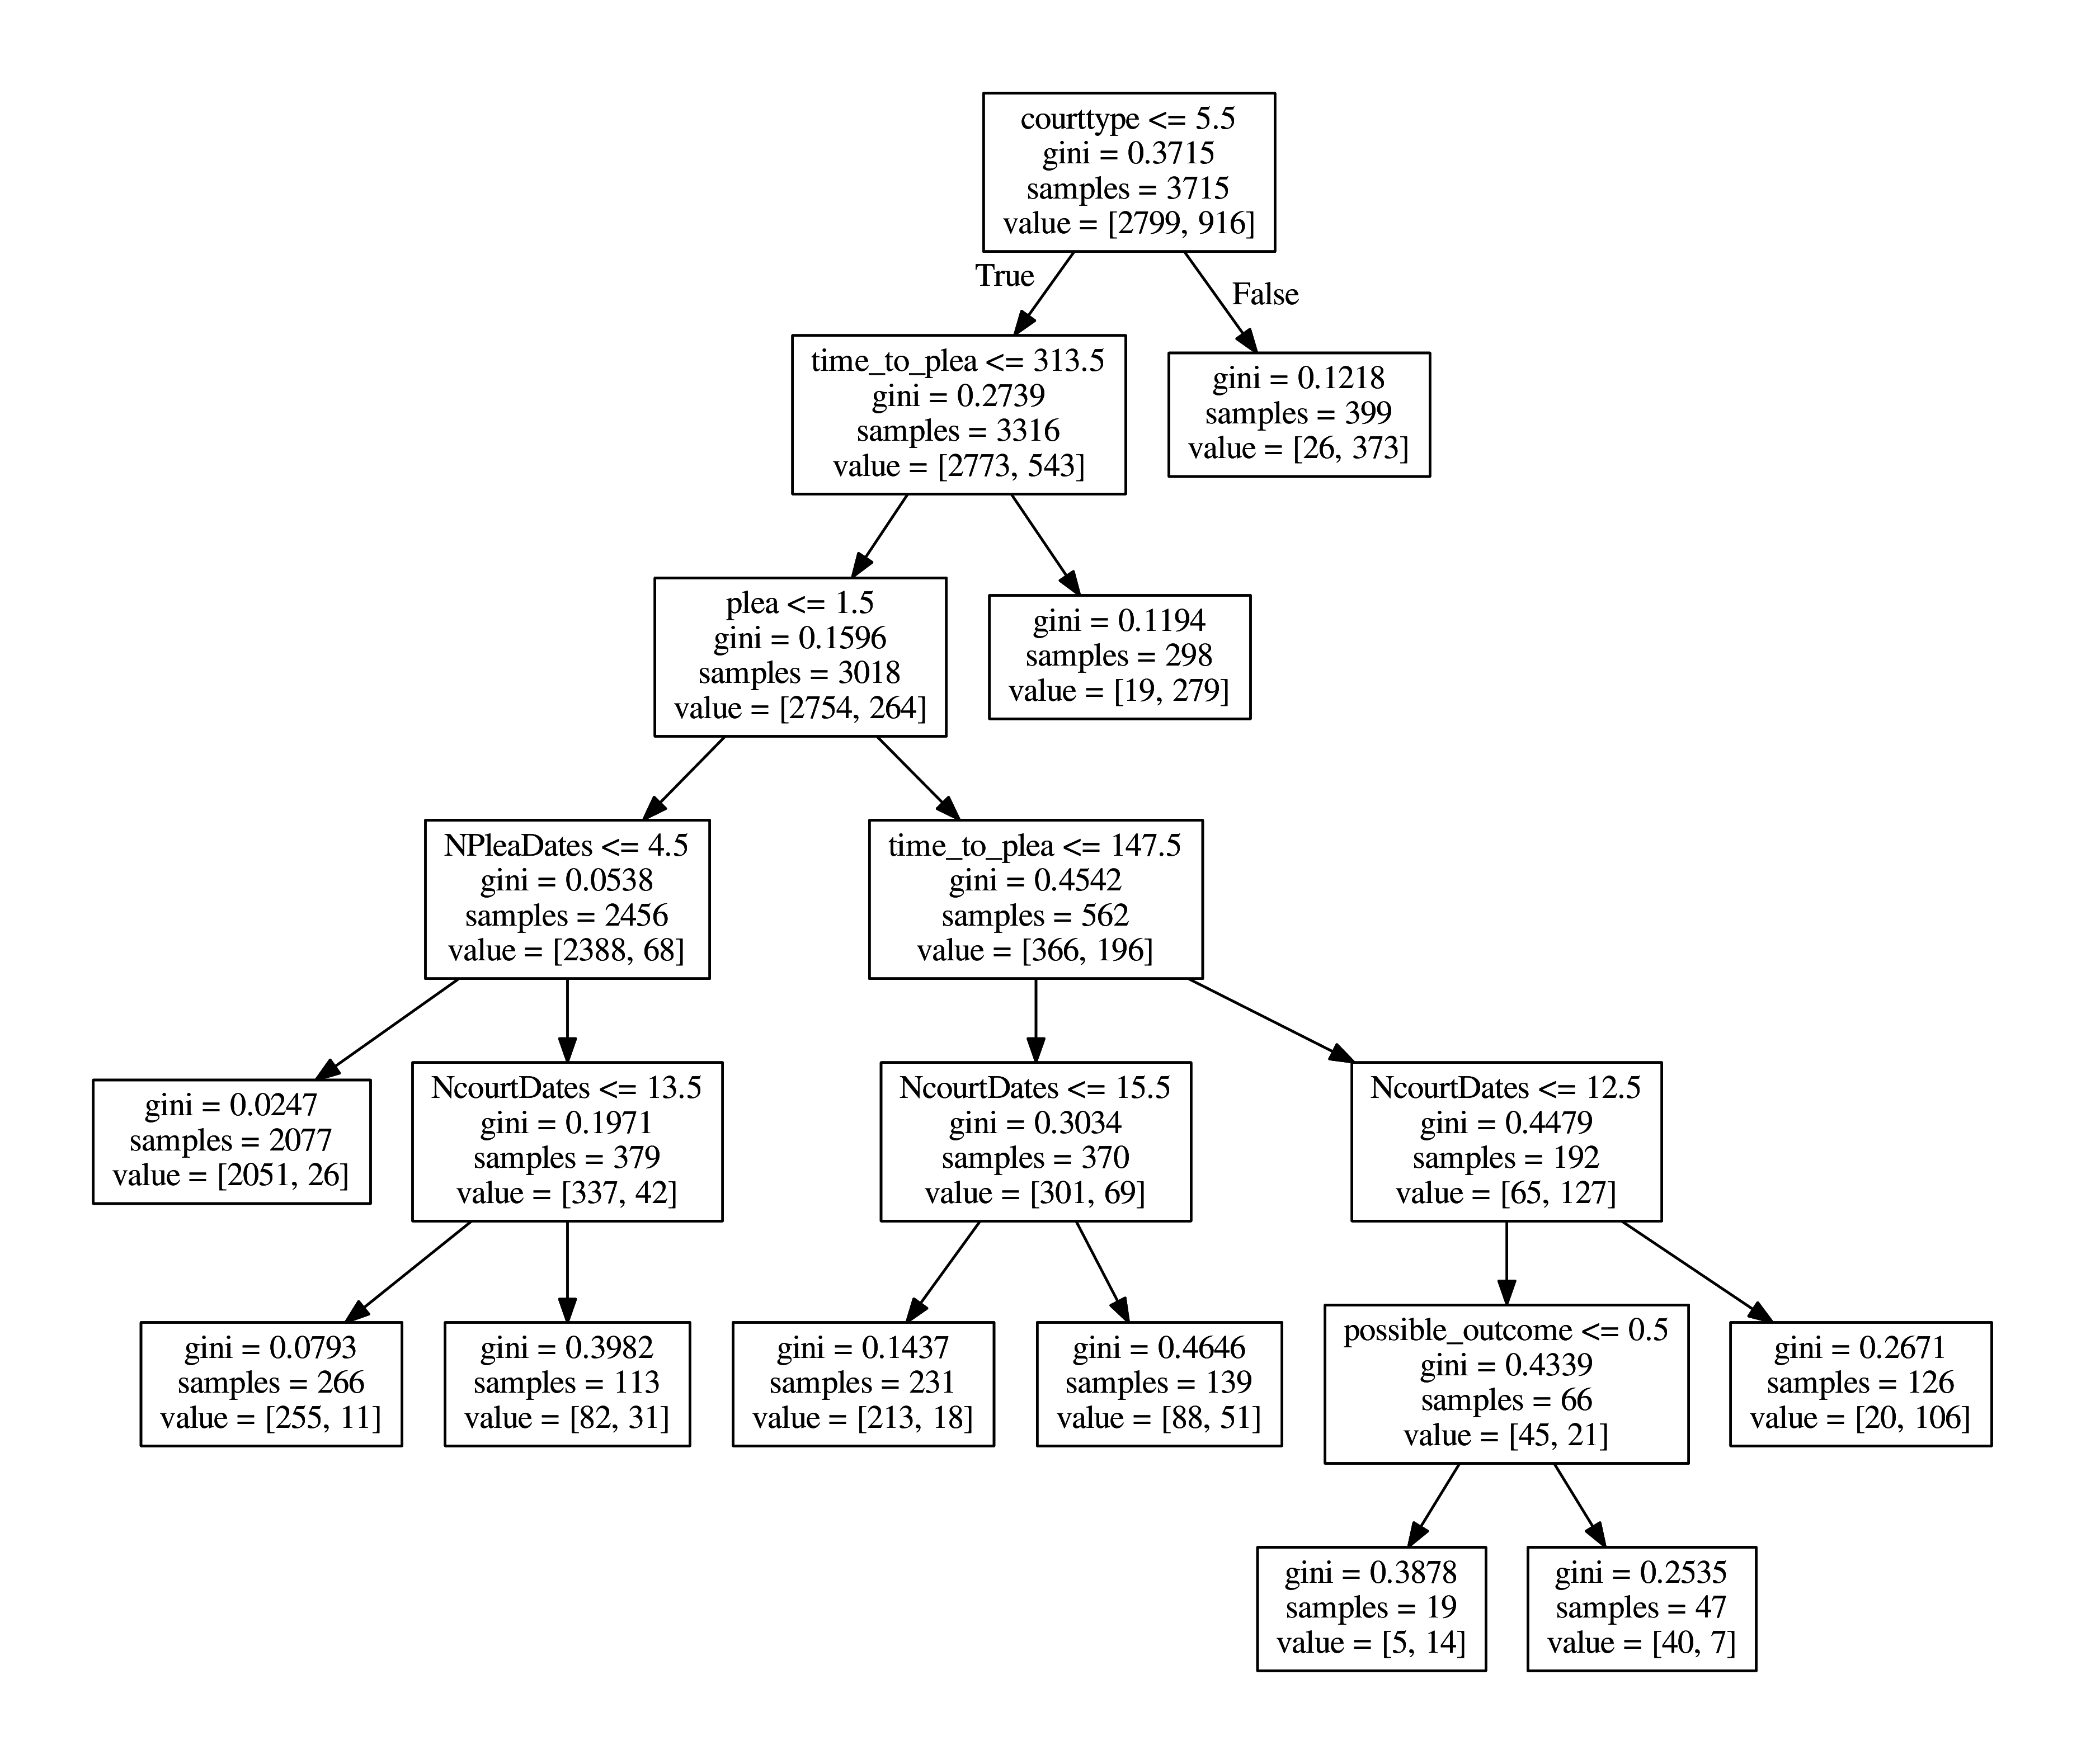
\includegraphics[width=0.70\columnwidth]{figures/simpleTree/simpleTree}
\caption{A single decision tree using the training data set, separating the data into the two classes "disposition less than one year" and "disposition greater than one year". At each decision node of the graph, the tree splits on the variable indicated, represented with two arrows drawn below it. The node indicates the boolean test on which the split is performed, the Gini coefficient (representing the purity of the node with respect to the final classification scheme), the number of samples on which the test is performed, and the size of each of the two true classifications. The data is split with the data for which the boolean test is True going to the left child node, and the data for which the boolean test is False going to the right child node. The performance of this tree would be evaluated by measuring how well it classifies a labeled test data set, using the final classifications in the terminal nodes (the "leaves" of the tree), which are assigned to the class having the larger number of observations in the population.
\label{fig:onetree}%
}
\end{center}
\end{figure}

\subsection{Leaf purity and feature importances}
The Gini impurity is calculated as the sum of the products of the population ratio and the classification error rate over each of $N$ classes,

$$I_{Gini} = \sum_{i=1}^{N}{p_i e_i}$$

with $p_{i}$ being the population ratio and $e_{i}$ being the misclassification rate, both for class $i$. In the case for $N=2$, this can be simplified: for a leaf having $a$ members in class 1 and $b$ members in class 2, the impurity can be calculated as

$$I_{Gini} = \frac{2 a b}{(a+b)^2}$$

For example, in the tree above, for the rightmost leaf on the bottom level that contains 40 classified in the first class and 7 in second class, the coefficient is calculated as $\frac{2 \times 40 \times 7}{(40+7)^2} = 0.2535$.

Leaf impurity measures can be used to determine which features of a decision tree model have the most importance to determining the final classifications. The Gini variable importance measure for a variable $X_m$ in a random forest of $N$ trees is given by \hyperref[csl:7]{(Louppe et al. 2013)}

$$Imp_{Gini}(X_m) = \frac{1}{N} \sum_T \sum_{t \in{T}: v(s_t)=X_m}{p(t)(I_{Gini}(t)-p_L I_{Gini}(t_L)-p_R I_{Gini}(t_R))}$$

where the summations are over all nodes $t$ in trees $T$ having $X_m$ as the splitting variable, $p(t)$ is the proportion of observations in the forest that are evaluated at node $t$, and $p_L$ and $p_R$ are the proportions of the population split to the left and right children nodes $t_L$ and $t_R$, respectively. We use this measure for variable importance throughout the rest of this paper.

In our analysis, the actual performance of the classification is less important than determining the variables that influence the classification. We evaluate the receiver operator characteristic (ROC) plots to validate that the models have some predictive power, but once that is established, the Gini variable importance measures are our primary interest. Weaknesses of this measure include a bias towards (higher reported values for) continuous variables and away (lower reported values for) variables with a small number of categories. It is also possible for a combination of lower importance variables to be jointly predictive, which would not be detected in a simple evaluation of importance rankings \hyperref[csl:8]{(Epifanio 2017)}.

\subsection{Treatment of categorical variables}
Categorical variables cannot be split at a tree node in a natural way, as a numerical or boolean variable can be. Two techniques are commonly used to transform categorical variables into other types: "one-hot encoding", which produces multiple boolean variables, one for each category; and a simple numerical mapping that assigns integers $i \in \{0, 1, ..., n-1\}$ to each of $n$ classes, such that each category gets a distinct integer label.

There are several weaknesses introduced with this method. For one-hot encoding, the observations within a single category become sparse which might undermine that category's importance. Also, one-hot encoded features of the original feature are dependent on each other. For the second method, by casting categories into integers we are imposing an order relationship to features that may not possess a natural sense of "greater than" or "less than". To counter this, the classification scheme can be permuted to determine if the order changes the outcomes.

To test how the choice of encoding scheme affects the resulting classification, we test a random forest using both methods and compare the resulting top feature importances. Here, one-hot encoding extends the feature space from 26 to 248 covariates. The second method performs the numerical cast on each of the categorical variables as described above, keeping the same number of covariates before and after the transformation. The results using these two schema are shown in Tables 3 and 4. We note that the order of the feature importances is similar between the two runs of the model, after observing that the features are themselves split in the one-hot encoded method. Because both methods (one hot encoding and casting categories into integers) give similar results, we take this to be a indicator of robustness with respect to classification choice, and in the remaining modeling we use only numerical classification.

\subsection{Random Forests}\label{rf} 
RFs are an ensemble learning method based on decision trees. The
prediction of the RF classifier is determined by majority voting
across multiple trees fit on subsamples of the data and subsamples of
the features.

We ran the RF model using four different sets of input variables. For
each we optimize the hyperparameters using a grid search routine from
the {\tt scikit-learn} python module \hyperref[csl:17]{(Pedregosa et
  al. 2011)}

In our first iteration, we use all of the engineered features. Using
hyperparameter grid-searching, we fit 50 trees with a minimum of 10
samples at each leaf node, each tree having a minimum of five
features, using a Gini impurity criterion (\autoref{gini}) to measure
leaf purity.

In order to detect disparities, we then recalibrate and run the RF
model with the demographic features removed. If the predictive power
increased with the inclusion of demographic variables (beyond the
expected increase due to a larger feature space), that would indicate
that these variables are influential on the model, and suggest the
presence of disparities in defendants' treatment based on demographic
information. We fit an RF classifier of 50 trees with a minimum of 2
samples at each leaf node, again with the Gini criteria. Each of these
trees considered a maximum of 20\% of the feature space.

Our third iteration of RFs is a classifier without timeline-related
features (see \autoref{tab:Features}). Having timeline-related
variables, such as time-to-plea, but also the number of court dates and
number of plea dates, as input features in the trees may be
problematic because of their correlation with the target
variable. Moreover, we hope to predict the length of cases with
information exogenous to the case proceedings; keeping
timeline-related variables in the classifier is helpful for pointing
out where delays may be happening during a case progression, but we
would also like to identify which features of our classifier become
important when runing without this retrospective information.

In the fourth model, we remove both the timeline-related variables and the
demographic variables, again comparing the performance of each to
identify any impact the demographic variables have on the resulting
classification.



\subsection{Gradient Boosted Decision Trees}

Whereas the RF is an ensemble learning method that operates on many
decision trees in parallel, the technique known as GBDT is an ensemble
method that operates on trees in a serial, recursive fashion.

Boosted models are constructed by adding many weak learners into a
single model, $$f_{M}(x) = \sum_{i=1}^{M}{T(x;\Theta_{i})}$$ where $M$
is the number of learners.  Generally, $T$ could be any type of
learner, but in a GBDT $T(x;\Theta_{i})$ is the $i$-th tree of the
model defined on the input variables $x$ and whose parameters
$\Theta_{i}$ define the structure of the tree. The $i+1$-th weak
learner is generated iteratively by fitting the tree on the residual
errors from the model of the first $i$ summed trees. In practice, this
is a difficult problem to solve analytically, so numerical methods are
substituted to estimate the next optimal tree. In the GBDT technique,
gradient descent is used to find the local minimum of the loss
function with respect to the current model. As with other
gradient-descent learning models, the rate of descent is an additional
hyperparameter to tune. The number of trees $M$ may be chosen
\textit{a priori} or be allowed to increase until the desired
performance is achieved.

Similarly to the RF models, we run the models four times using the
same variable sets as identified above, using the same grid-search
algorithm to optimize the hyperparameters of the model.


\begin{figure}[h!]
\begin{center}
\includegraphics[width=0.70\columnwidth]{figures/pasted_image_at_2017_07_29_09_16_pm/Pasted_image_at_2017_07_30_07_23_PM}
\caption{Top ten feature importances for each of the models run for random forest (panels on left, (\textit{a}), (\textit{c}), (\textit{e}) and (\textit{g})) and gradient boosted trees (panels on right, (\textit{b}), (\textit{d}), (\textit{f}) and (\textit{h})). 
\label{fig:featureimportances}%
}
\end{center}
\end{figure}

\begin{figure}[h!]
\begin{center}
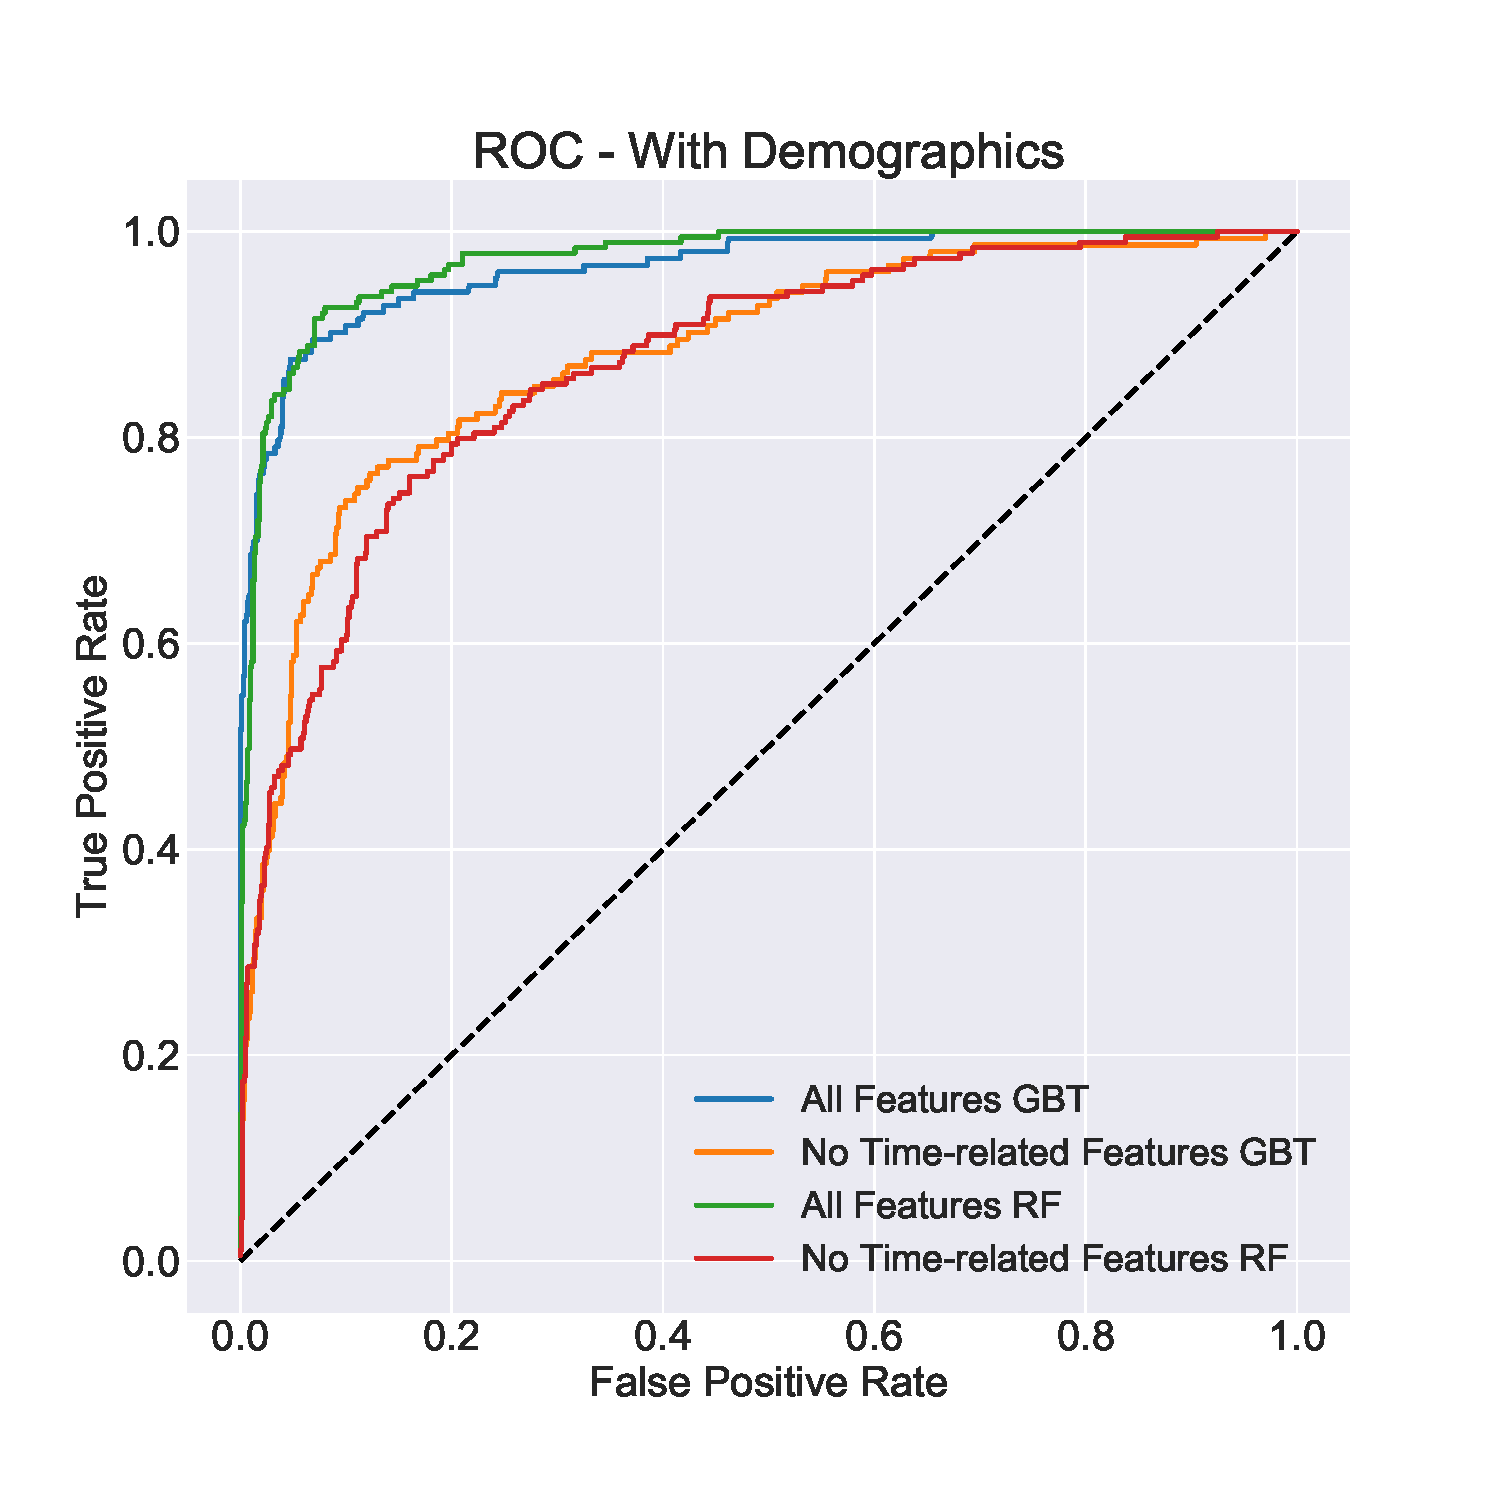
\includegraphics[width=0.70\columnwidth]{figures/roc_curve_rf2/ROC_wdemo}
\caption{ROC curves for the RF and GBT models, with the addition of Demographic Data. The ROC plots show True Positive (completeness) {\it vs} False Positive rate (purity) of a classifier. The ROCs change slightly depending on the subset of variables in the model. The two ensemble methods exhibit similar performance. The addition of the Time-Related features improve the accuracy of the predictions and therefore we infer that they are important covariates for the prediction of long duration dispositions.
\label{fig:demoROC}%
}
\end{center}
\end{figure}

\begin{figure}[h!]
\begin{center}
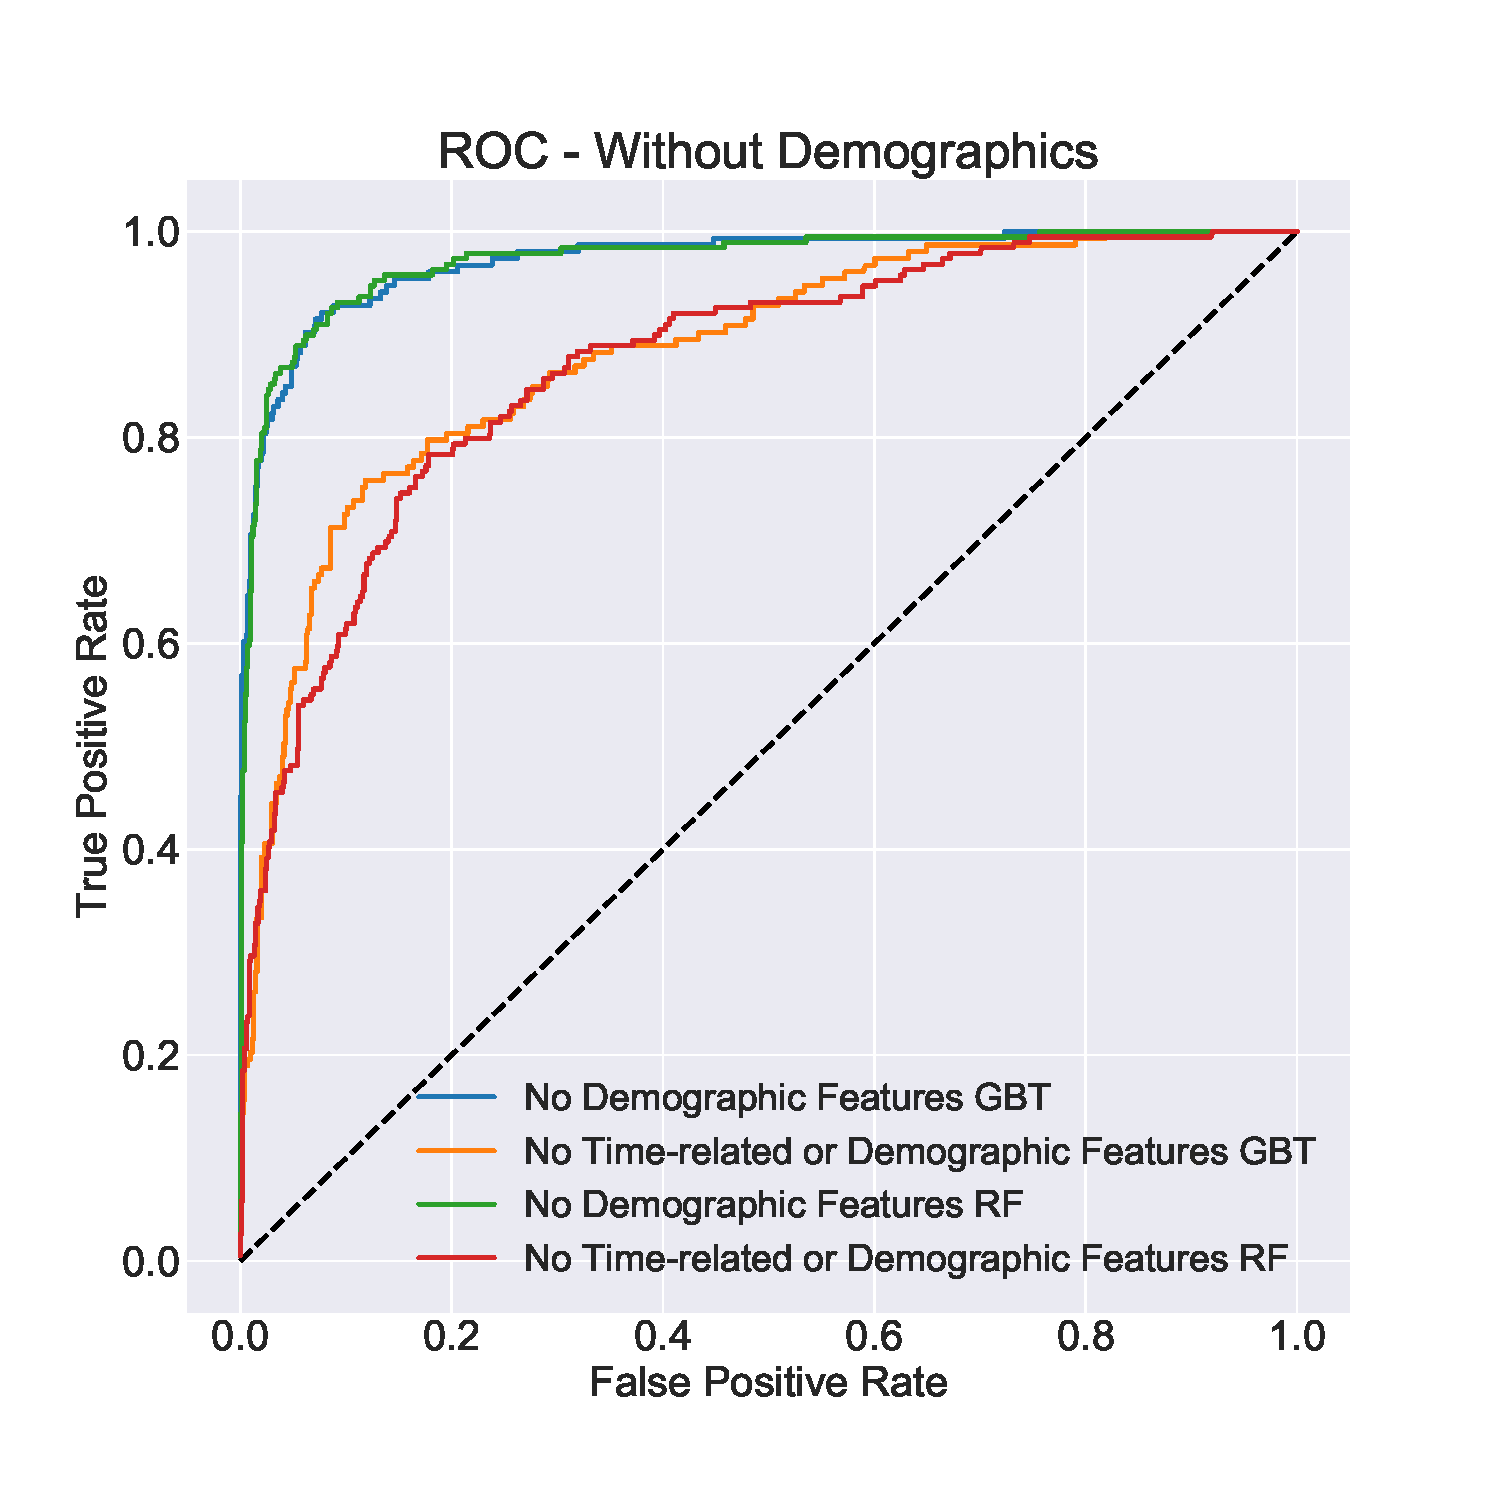
\includegraphics[width=0.70\columnwidth]{figures/ROC_without_demographics1/ROC_nodemo}
\caption{ROC curves for the RF and GBT models, without the addition of Demographic Data. A change in the shape of the plots between this and Fig. \ref{fig:demoROC} (including demographics) would indicate a change in the predictive power; however we do not observe that here. This suggests that there is no evidence of significant disparities with the inclusion of the demographic data.
\label{fig:nodemoROC}%
}
\end{center}
\end{figure}

\section{Appendix}
% Please add the following required packages to your document preamble:
% \usepackage{booktabs}
\begin{table*}[]
\centering
\tiny
\begin{tabular}{@{}ccccc@{\qquad}cccc@{}}
\cmidrule(r){2-5} \cmidrule(l){7-10}
                          & \multicolumn{4}{c}{Random Forest}                                                            & \multicolumn{4}{c}{Gradient Boosted Tree}                                                  \\ \cmidrule(r){2-5} \cmidrule(l){7-10} 
                          & \multicolumn{2}{c}{With time-dependant vars} & \multicolumn{2}{c}{W/o time-dependant vars}   & \multicolumn{2}{c}{With time-dependant vars} & \multicolumn{2}{c}{W/o time-dependant vars} \\
                          & w/ Demogr.            & w/o Demog.           & w/ Demogr.           & w/o Demog.             & w/ Demogr.            & w/o Demog.           & w/ Demogr.           & w/o Demog.           \\
Age at Offense            & 0.011                 & --                   & 0.04                 & --                     & 0.042                 & --                   & 0.062                & --                   \\
Court Type                & 0.03                  & 0.031                & 0.09                 & 0.098                  & 0.054                 & 0.048                & 0.056                & 0.073                \\
Courtroom Count           & 0.018                 & 0.018                & 0.078                & 0.087                  & 0.032                 & 0.045                & 0.079                & 0.092                \\
Enhancement PC 12022      & 0.003                 & 0.003                & 0.012                & 0.015                  & 0                     & 0                    & 0.003                & 0                    \\
Enhancement PC 1368       & 0.001                 & 0                    & 0.004                & 0.004                  & 0.002                 & 0.002                & 0.028                & 0.032                \\
Gang Enhancement          & 0                     & 0                    & 0.002                & 0.002                  & 0.002                 & 0.002                & 0.002                & 0                    \\
Gender                    & 0.002                 & --                   & 0.006                & --                     & 0                     & --                   & 0.008                & --                   \\
In custody                & 0.013                 & 0.013                & 0.036                & 0.039                  & 0.018                 & 0.021                & 0.045                & 0.052                \\
Initial Plea              & 0.08                  & 0.08                 & 0.222                & 0.236                  & 0.059                 & 0.057                & 0.054                & 0.055                \\
Main Charge               & 0.013                 & 0.013                & 0.051                & 0.06                   & 0.077                 & 0.072                & 0.151                & 0.191                \\
No. Charges               & 0.006                 & 0.006                & 0.021                & 0.026                  & 0.024                 & 0.032                & 0.011                & 0.019                \\
No. Court Dates           & 0.155                 & 0.161                & --                   & --                     & 0.167                 & 0.182                & --                   & --                   \\
No. Defendants            & 0.003                 & 0.003                & 0.011                & 0.014                  & 0.005                 & 0.006                & 0.005                & 0.006                \\
No. Enhancements          & 0.007                 & 0.007                & 0.028                & 0.032                  & 0.005                 & 0.016                & 0.012                & 0.021                \\
No. Failures to Appear    & 0.006                 & 0.006                & 0.036                & 0.04                   & 0.019                 & 0.014                & 0.044                & 0.057                \\
No. Felony Charges        & 0.014                 & 0.012                & 0.051                & 0.059                  & 0.022                 & 0.021                & 0.079                & 0.087                \\
No. Health Code Charges   & 0.006                 & 0.006                & 0.017                & 0.022                  & 0.006                 & 0.011                & 0.036                & 0.055                \\
No. Penal Code Charges    & 0.008                 & 0.008                & 0.029                & 0.034                  & 0.034                 & 0.043                & 0.031                & 0.042                \\
No. Plea Dates            & 0.1                   & 0.1                  & --                   & --                     & 0.024                 & 0.037                & --                   & --                   \\
No. Vehicle Code Charges  & 0.001                 & 0.001                & 0.004                & 0.005                  & 0.003                 & 0.005                & 0.011                & 0.021                \\
Possible Sentence Outcome & 0.029                 & 0.029                & 0.097                & 0.105                  & 0.051                 & 0.065                & 0.081                & 0.087                \\
Preliminary Hearing       & 0.052                 & 0.053                & --                   & --                     & 0.006                 & 0.011                & --                   & --                   \\
Public Defender           & 0.002                 & 0.002                & 0.005                & 0.006                  & 0.014                 & 0.013                & 0.006                & 0.011                \\
Race/Ethnicity            & 0.005                 & --                   & 0.017                & --                     & 0.014                 & --                   & 0.023                & --                   \\
Time Waived               & 0.006                 & 0.006                & 0.021                & 0.025                  & 0.008                 & 0.01                 & 0.039                & 0.049                \\
Time to Plea              & 0.396                 & 0.42                 & --                   & --                     & 0.229                 & 0.242                & --                   & --                   \\
Trial                     & 0.004                 & 0.004                & 0.013                & 0.016                  & 0                     & 0                    & 0.002                & 0.002                \\
Type of Defense Attorney  & 0.017                 & 0.017                & 0.066                & 0.074                  & 0.043                 & 0.046                & 0.042                & 0.047                \\
Zip Code                  & 0.013                 & --                   & 0.043                & --                     & 0.038                 & --                   & 0.09                 & --                   \\ \cmidrule(r){2-5} \cmidrule(l){7-10} 
\end{tabular}
\caption{Feature importances found for each of the eight runs of models. ``--'' indicates the variable was not used in the model.}
\label{tab:featimp}
\end{table*}

\selectlanguage{english}
\FloatBarrier
\section*{References}\sloppy
\phantomsection
\label{csl:1}Katz, Daniel Martin, Michael J. Bommarito Ii, and Josh Blackman. 2017. ``{A General Approach for Predicting the Behavior of the {Supreme} {Court} of the {United} {States}}''. \textit{PLOS ONE} 12 (4): e0174698. \url{https://doi.org/10.1371/journal.pone.0174698.}

\phantomsection
\label{csl:2}Lakkaraju, Himabindu, and Cynthia Rudin. 2016. ``{Learning {Cost}-{Effective} and {Interpretable} {Regimes} for {Treatment} {Recommendation}}''. In \textit{{ArXiv}:1611.07663 [Stat]}. Barcelona, Spain. \url{http://arxiv.org/abs/1611.07663.}

\phantomsection
\label{csl:3}Walt, Stéfan van der, and Nathaniel Smith. 2015. ``{Matplotlib Colormaps}''. \url{http://bids.github.io/colormap/.}

\phantomsection
\label{csl:4}James, Gareth, Daniela Witten, Trevor Hastie, and Robert Tibshirani. 2013. \textit{{An Introduction to Statistical Learning}}. Springer New York. \url{https://doi.org/10.1007/978-1-4614-7138-7.}

\phantomsection
\label{csl:5}Pedregosa, F., G. Varoquaux, A. Gramfort, V. Michel, B. Thirion, O. Grisel, M. Blondel, et al. 2011. ``{Scikit-Learn: Machine Learning in {P}Ython}''. \textit{Journal of Machine Learning Research} 12: 2825–30.

\phantomsection
\label{csl:6}Chen, Tianqi, and Carlos Guestrin. 2016. ``{XGBoost}''. In \textit{Proceedings of the 22nd {ACM} {SIGKDD} International Conference on Knowledge Discovery and Data Mining - {KDD} {\Textquotesingle}16}. {ACM} Press. \url{https://doi.org/10.1145/2939672.2939785.}

\phantomsection
\label{csl:7}Louppe, Gilles, Louis Wehenkel, Antonio Sutera, and Pierre Geurts. 2013. ``{Understanding Variable Importances in Forests of Randomized Trees}''. In \textit{Advances in Neural Information Processing Systems 26}, edited by C. J. C. Burges, L. Bottou, M. Welling, Z. Ghahramani, and K. Q. Weinberger, 431–39. Curran Associates, Inc. \url{http://papers.nips.cc/paper/4928-understanding-variable-importances-in-forests-of-randomized-trees.pdf.}

\phantomsection
\label{csl:8}Epifanio, Irene. 2017. ``{Intervention in Prediction Measure: a New Approach to Assessing Variable Importance for Random Forests}''. \textit{{BMC} Bioinformatics} 18 (1). \url{https://doi.org/10.1186/s12859-017-1650-8.}

\end{document}

